\documentclass[a4paper, 12pt]{article}
\usepackage{lmodern}
\usepackage{amssymb,amsmath}
\usepackage{ifxetex,ifluatex}
\usepackage{fixltx2e} % provides \textsubscript
\ifnum 0\ifxetex 1\fi\ifluatex 1\fi=0 % if pdftex
  \usepackage[T1]{fontenc}
  \usepackage[utf8]{inputenc}
\else % if luatex or xelatex
  \ifxetex
    \usepackage{mathspec}
  \else
    \usepackage{fontspec}
  \fi
  \defaultfontfeatures{Ligatures=TeX,Scale=MatchLowercase}
\fi
% use upquote if available, for straight quotes in verbatim environments
\IfFileExists{upquote.sty}{\usepackage{upquote}}{}
% use microtype if available
\IfFileExists{microtype.sty}{%
\usepackage{microtype}
\UseMicrotypeSet[protrusion]{basicmath} % disable protrusion for tt fonts
}{}
\usepackage[left=3.5cm,right=2.5cm,top=2.5cm,bottom=2.5cm]{geometry}
\usepackage{hyperref}
\PassOptionsToPackage{usenames,dvipsnames}{color} % color is loaded by hyperref
\hypersetup{unicode=true,
            pdftitle={Avaliação pela Moda, Média ou Mediana?},
            pdfauthor={Luiz Fernando Palin Droubi; Norberto Hochheim; Willian Zonato},
            colorlinks=true,
            linkcolor=red,
            citecolor=green,
            urlcolor=magenta,
            breaklinks=true}
\urlstyle{same}  % don't use monospace font for urls
\usepackage{longtable,booktabs}
\usepackage{graphicx,grffile}
\makeatletter
\def\maxwidth{\ifdim\Gin@nat@width>\linewidth\linewidth\else\Gin@nat@width\fi}
\def\maxheight{\ifdim\Gin@nat@height>\textheight\textheight\else\Gin@nat@height\fi}
\makeatother
% Scale images if necessary, so that they will not overflow the page
% margins by default, and it is still possible to overwrite the defaults
% using explicit options in \includegraphics[width, height, ...]{}
\setkeys{Gin}{width=\maxwidth,height=\maxheight,keepaspectratio}
\IfFileExists{parskip.sty}{%
\usepackage{parskip}
}{% else
\setlength{\parindent}{0pt}
\setlength{\parskip}{6pt plus 2pt minus 1pt}
}
\setlength{\emergencystretch}{3em}  % prevent overfull lines
\providecommand{\tightlist}{%
  \setlength{\itemsep}{0pt}\setlength{\parskip}{0pt}}
\setcounter{secnumdepth}{5}
% Redefines (sub)paragraphs to behave more like sections
\ifx\paragraph\undefined\else
\let\oldparagraph\paragraph
\renewcommand{\paragraph}[1]{\oldparagraph{#1}\mbox{}}
\fi
\ifx\subparagraph\undefined\else
\let\oldsubparagraph\subparagraph
\renewcommand{\subparagraph}[1]{\oldsubparagraph{#1}\mbox{}}
\fi

%%% Use protect on footnotes to avoid problems with footnotes in titles
\let\rmarkdownfootnote\footnote%
\def\footnote{\protect\rmarkdownfootnote}

%%% Change title format to be more compact
\usepackage{titling}

% Create subtitle command for use in maketitle
\newcommand{\subtitle}[1]{
  \posttitle{
    \begin{center}\large#1\end{center}
    }
}

\setlength{\droptitle}{-2em}

  \title{Avaliação pela Moda, Média ou Mediana?}
    \pretitle{\vspace{\droptitle}\centering\huge}
  \posttitle{\par}
  \subtitle{Teoria e simulações}
  \author{Luiz Fernando Palin Droubi\footnote{SPU/SC,
  \href{mailto:luiz.droubi@planejamento.gov.br}{\nolinkurl{luiz.droubi@planejamento.gov.br}}} \\ Norberto Hochheim\footnote{UFSC,
  \href{mailto:hochheim@gmail.com}{\nolinkurl{hochheim@gmail.com}}} \\ Willian Zonato\footnote{SPU/SC,
  \href{mailto:willian.zonato@planejamento.gov.br}{\nolinkurl{willian.zonato@planejamento.gov.br}}}}
    \preauthor{\centering\large\emph}
  \postauthor{\par}
      \predate{\centering\large\emph}
  \postdate{\par}
    \date{31/10/2018}

\usepackage[brazil]{babel}
\usepackage{graphicx}
\usepackage{float}
\usepackage{subfig}
\usepackage{caption}
\usepackage{lastpage}
\setlength{\parindent}{1.25cm} % Default is 15pt.
\usepackage{indentfirst}
\usepackage{fontspec} % para Arial
\setmainfont{Arial}
\newcommand{\pkg}[1]{{\normalfont\fontseries{b}\selectfont #1}}
\let\proglang=\textsf
\let\code=\texttt
\usepackage{fancyhdr}
% Turn on the style
\pagestyle{fancy}
% Clear the header and footer
\fancyhead{}
\fancyfoot{}
% Set the right side of the footer to be the page number
\fancyfoot[R]{\thepage~/~\pageref{LastPage}}
\usepackage{booktabs}
\usepackage{longtable}
\usepackage{array}
\usepackage{multirow}
\usepackage[table]{xcolor}
\usepackage{wrapfig}
\usepackage{float}
\usepackage{colortbl}
\usepackage{pdflscape}
\usepackage{tabu}
\usepackage{threeparttable}
\usepackage{threeparttablex}
\usepackage[normalem]{ulem}
\usepackage{makecell}

\begin{document}
\maketitle

\section{INTRODUÇÃO}\label{introducao}

Existe na área da avaliação de imóveis uma discussão frequente e a nosso
ver indesejável a respeito da estimativa de tendência central adotada
para a predição de valores quando da utilização de modelos lineares
log-normais, isto é, modelos em que a variável resposta aparece
transformada pela função logaritmo natural.

Como será visto oportunamente, quando um modelo linear log-normal for
homocedástico (\(\sigma=cte\)) e estiver razoavelmente bem ajustado, com
um baixo erro-padrão, a adoção de qualquer estimativa de tendência
central, moda, média ou mediana, resultará em valores praticamente
equivalentes com variação dentro da precisão da área de avaliações
imobiliárias. No entanto, na presença de grande dispersão dos dados, o
valor do erro-padrão da regressão linear pode se tornar relativamente
alto e a diferença entre as avaliação por uma ou outra medida de
tendência central pode tornar-se relevante, levando a uma situação
altamente indesejável: um imóvel poderá ser avaliado por dois
avaliadores independentes com uma diferença significativa entre os
valores encontrados. Tendo em vista que a NBR14.653-02
(\protect\hyperlink{ref-NBR1465302}{2011}) se omite a este respeito, as
duas avaliações serão válidas, porém com valores altamente discrepantes.

Pretende-se com este artigo dar a este problema uma abordagem formal,
com o intuito de sugerir uma padronização das avaliações, sem no entanto
especificar qual medida de tendência central é a correta, haja vista que
todas elas tem seus prós e contras e nenhuma delas pode ser dita melhor
do que a outra.

\section{DESENVOLVIMENTO E
FUNDAMENTAÇÃO}\label{desenvolvimento-e-fundamentacao}

\begin{quote}
Major Point 1: When we talk about the relationship of one variable to
one or more others, we are referring to the regression function, which
expresses the mean of the first variable as a function of the others.
The key word here is \emph{mean}! (MATLOFF,
\protect\hyperlink{ref-matloff2009}{2009}, p. 386, grifo do autor)
\end{quote}

\subsection{Valor Esperado}\label{valor-esperado}

Segundo BENNETT (\protect\hyperlink{ref-bennett}{2006}), a
\textbf{esperança matemática} ou \textbf{valor esperado } de uma
variável aleatória é a soma do produto de cada probabilidade de saída da
experiência pelo seu respectivo valor. Isto é, representa o valor médio
`esperado' de uma experiência se ela for repetida muitas vezes.
Matematicamente, a Esperança de uma variável aleatória \(X\) é
representada pelo símbolo \(\mathbb{E}(X)\)

Segundo Matloff (\protect\hyperlink{ref-matloff2009}{2009}, p. 43), o
valor esperado tem um papel central em probabilidade e estatística. A
definição mais ampla de valor esperado de uma variável aleatória \(X\),
válida tanto para variáveis discretas como contínuas, é:

\[\lim_{n \to \infty} = \frac{X_1 + \ldots + X_n}{n}\]

\subsubsection{Cômputo do Valor Esperado de uma variável aleatória
discreta}\label{computo-do-valor-esperado-de-uma-variavel-aleatoria-discreta}

Segundo Matloff (\protect\hyperlink{ref-matloff2009}{2009}, p. 44), o
valor esperado de uma variável aleatória \(X\) que assume valores
definidos no conjunto \(A\) é:

\[\mathbb{E}(X) = \sum_{c \in A}c\mathbb{P}(X=c)\]

onde \(\mathbb{P(X = c)}\) representa a função probabilidade da variável
aleatória \(X\) assumir o valor \(c\).

\subsubsection{Cômputo do Valor Esperado de uma variável aleatória
contínua}\label{computo-do-valor-esperado-de-uma-variavel-aleatoria-continua}

O Valor Esperado de uma variável aleatória contínua \(W\) pode ser
escrito da seguinte forma (MATLOFF,
\protect\hyperlink{ref-matloff2009}{2009}, p. 128)

\[\mathbb{E}(W) = \int_{-\infty}^{\infty}tf_W(t)dt\]

onde \(f_W(t)\) é a função densidade de probabilidade de \(t\), para
todo \(t\) onde a função \(f_W(t)\) esteja definida.

\subsubsection{Propriedades do Valor
Esperado}\label{propriedades-do-valor-esperado}

Seja \(a\) um escalar e \(U\) uma variável aleatória (MATLOFF,
\protect\hyperlink{ref-matloff2017}{2017}, p. 47):

\[\mathbb{E}(aU) = a\mathbb{E}(U)\]

Sejam \(a\) e \(b\) dois escalares e \(U\) e \(V\) duas variáveis
aleatórias, não necessariamente independentes, então (MATLOFF,
\protect\hyperlink{ref-matloff2017}{2017}, p. 47):

\[\mathbb{E}(aU + bV) = a\mathbb{E}(U) + bE(V)\]

Finalmente, sejam \(U\) e \(V\) duas variáveis aleatórias
\emph{independentes}:

\[\mathbb{E}(UV) = \mathbb{E}(U)\mathbb{E}(V)\]

Porém, se \(U\) e \(V\) não forem independentes, esta propriedade falha
(covariância).

\subsubsection{Lei da expectativa total}\label{lei-da-expectativa-total}

Segundo Matloff (\protect\hyperlink{ref-matloff2009}{2009}, p. 339), a
lei da expectativa total pode ser expressa como abaixo:

\[\mathbb{E}(Y) = \mathbb{E}[\mathbb{E}(Y|W)]\]

\subsubsection{Lei da Variância total}\label{lei-da-variancia-total}

Outra relação importante é expressa pela lei da Variância Total que, de
acordo com Matloff (\protect\hyperlink{ref-matloff2009}{2009}, p. 345)
estabelece que:

\[\text{Var}(Y) = \mathbb{E}[\text{Var}(Y|W)] + \text{Var}[\mathbb{E}(Y|W)]\]

\subsection{Desigualdade de Jensen}\label{desigualdade-de-jensen}

Segundo Matloff (\protect\hyperlink{ref-matloff2017}{2017}), se
\(\varphi(x)\) é uma função convexa, então a desiguldade de Jensen se
exprime na seguinte desigualdade:

\(\varphi \left(\mathbb{E} [X]\right)\leq \mathbb{E} \left[\varphi (X)\right].\)

Como pode-se demonstrar, a função \(e^x\) é uma função convexa, pois
possui derivada segunda sempre maior que zero (\({f}''=e^x>0\)).

\subsubsection{Erro médio quadrático
(MSE)}\label{erro-medio-quadratico-mse}

Seja \(\pi\) o valor de uma estimativa. Então o seu erro médio
quadrático (MSE) é dado por:

\[\text{MSE} = \int(y - \pi)f(y)dy\\
= \mathbb{E}[(y-\pi)^2]\\
= \mathbb{E}(y^2)-2\pi \mathbb{E}(y)+\pi^2\]

Para encontrar o valor mínimo do erro médio quadrático (MSE) quando
\(\pi\) varia, faz-se:

\[\frac{d(\mathbb{E}(y^2)-2\pi \mathbb{E}(y)+\pi^2)}{d\pi} = 0\\
\therefore \pi = \mathbb{E}(y)\]

Ou seja, a estimativa pelo valor esperado é a estimativa que minimiza e
erro médio quadrático.

\subsubsection{Valor Esperado
condicional}\label{valor-esperado-condicional}

O valor esperado de uma variável aleatória \(Y\) estatisticamente
relacionada com outra outra variável aleatória \(X\) é (WASSERMAN,
\protect\hyperlink{ref-wasserman}{2010}, p. 77):

\[\mathbb{E}(Y|X = t) = \int{t} f_{Y|X}(Y|X = t)dt\]

\subsection{Estimadores}\label{estimadores}

\begin{quote}
Earlier, we often referred to certain estimators as being ``natural.''
For example, if we are estimating a population mean, an obvious choice
of estimator would be the sample mean. But in many applications, it is
less clear what a ``natural'' estimate for a population quantity of
interest would be. We will present general methods for estimation in
this section. We will also discuss advanced methods of inference
(MATLOFF, \protect\hyperlink{ref-matloff2009}{2009}, p. 303).
\end{quote}

A definição de um \emph{estimador} para um parâmetro ou uma variável
\(\theta\) é uma função \(\hat{\theta}(X)\), que mapeia o espaço
amostral para um conjunto de estimativas amostrais, em que \(X\) é uma
variável aleatória dos dados observados. É usual denotar uma estimativa
em um determinado ponto \(x \in X\) por \(\hat{\theta}(X = x)\) ou, mais
simplesmente, \(\hat{\theta}(x)\).

\subsubsection{Propriedades de um
estimador}\label{propriedades-de-um-estimador}

Nesta seção adota-se que \(\hat{\theta}\) é um estimador da variável
aleatória \(\theta\).

\paragraph{Erro}\label{erro}

\[e(x) = \hat{\theta}(x) - \theta\]

\paragraph{Desvio}\label{desvio}

\[d(x) = \hat{\theta}(x) - \mathbb{E}(\hat{\theta}(X))\] onde
\(\mathbb{E}(\hat{\theta}(X))\) é o Valor Esperado do estimador.

\paragraph{Variância}\label{variancia}

A variância de um estimador \(\theta\) é (MATLOFF,
\protect\hyperlink{ref-matloff2009}{2009}, p. 52):

\[\text{Var}(\hat{\theta}) = \mathbb{E}[(\hat{\theta} - \mathbb{E}[\hat{\theta}])^2]\]

\paragraph{Coeficiente de Variação}\label{coeficiente-de-variacao}

O coeficiente de variação de um estimador é uma medida adimensional que
compara o desvio-padrão de uma variável ou estimador \(\theta\) à sua
média, conforme abaixo (MATLOFF,
\protect\hyperlink{ref-matloff2009}{2009}, p. 56):

\[CV = \frac{\sqrt{\text{Var}(\hat{\theta})}}{E[\hat{\theta}]}\]

\paragraph{Viés}\label{vies}

O viés de um estimador \(\hat{\theta}\) é (MATLOFF,
\protect\hyperlink{ref-matloff2009}{2009}, p. 317):

\[\text{B}(\hat{\theta}) = \mathbb{E}[\hat{\theta}] - \theta\]

O viés coincide com o valor esperado do erro, pois
\(\mathbb{E}(\hat{\theta}) - \theta = \mathbb{E}(\hat{\theta}-\theta)\).

Numa regressão linear:

\[\text{B}[\hat{\mu}(x_0)] = \mathbb{E}[\hat{\mu}(x_0)] - \mu(x_0)\]

\paragraph{Erro médio quadrático}\label{erro-medio-quadratico}

Segundo Shen e Zhu (\protect\hyperlink{ref-shen}{2008}, p. 553), o erro
médio quadrático é uma medida comum da qualidade de um estimador na
literatura estatística.

\[\text{MSE} = \mathbb{E}[(\hat{\theta} - \theta)^2]\]

Numa regressão linear, o erro médio quadrático pode ser descrito por:

\[\text{MSE}[\hat{\mu}(x_0)] = \mathbb{E}[\hat{\mu}(x_0) - \mu(x_0)]^2 = \text{Var}[\hat{\mu}(x_0)] + \text{B}^2[\hat{\mu}(x_0)]\]

\paragraph{Consistência}\label{consistencia}

\[\lim_{n \rightarrow \infty}\hat{\theta} = \theta\]

\subsubsection{Melhor estimador linear não-viesado ou
BLUE}\label{melhor-estimador-linear-nao-viesado-ou-blue}

Em estatística, é comum o uso da sigla BLUE (\emph{Best Linear Unbiased
Estimator}) para indicar o melhor estimador linear não-viesado.

\subsubsection{Trade-off entre viés e
variância}\label{trade-off-entre-vies-e-variancia}

Um dos problemas conhecidos dos modelos de regressão linear ou outros
modelos estatísticos em geral é o sobreajustamento (do inglês
\emph{overfitting}). Resumidamente, \emph{overfitting} é o ato de
ajustar um modelo tão bem ajustado aos dados amostrais, que este se
torna incapaz de fazer boas previsões para outros dados que não os do
modelo. Segundo Matloff (\protect\hyperlink{ref-matloff2017}{2017}, p.
24), um modelo sobreajustado é um modelo tão elaborado que ``capta o
ruído ao invés do sinal''.

Segundo Matloff (\protect\hyperlink{ref-matloff2017}{2017}, pp. 24--26),
pelo contrário, um modelo com menor número de variáveis explicativas
estará enviesando os seus resultados (no sentido de enviesamento
sistêmico, inerente à amostragem, não proposital), e o acréscimo de uma
variável independente a este modelo estará assim reduzindo o seu viés.

Por outro lado, de acordo com Matloff
(\protect\hyperlink{ref-matloff2017}{2017}, p. 25), quanto maior for o
número de variáveis do modelo -- mantido o mesmo número de dados
amostrais --, maior será a variabilidade coletiva dos regressores e,
assim, maior será a variância dos coeficientes estimados.

Desta maneira, em modelos mais simples, a redução do viés do mesmo
através da adição de um novo regressor compensa o aumento na
variabilidade conjunta do modelo, até que este número de regressores
atinja um número ótimo, quando a diminuição adicional do viés gerada
pela adição de um regressor torna-se tão pequena que não compensa a
variabilidade dos coeficientes estimados. Um modelo com variáveis
explicativas maior do que este número ótimo estará, portanto,
sobreajustado.

Ou seja, existe um \emph{tradeoff} entre viés e variância: para qualquer
estimador estatístico (MATLOFF,
\protect\hyperlink{ref-matloff2017}{2017}, p. 25), não se pode reduzir o
seu viés sem aumentar a sua variância e vice-versa. Tem-se que conviver
sempre com algum viés e tem que se aceitar alguma variância.

Matematicamente, isto decorre do desenvolvimento da expressão do Erro
Médio Quadrático (MSE) (MATLOFF,
\protect\hyperlink{ref-matloff2017}{2017}, p. 49):

\[\mathbb{E}[(\hat{\theta} - \theta)^2] = \mathbb{E}[\hat{\theta} - \mathbb{E}[\hat{\theta}] + \mathbb{E}[\hat{\theta}] - \theta]^2\]

Desenvolvendo a expressão acima, chega-se:

\[\text{MSE} = \mathbb{E}[(\hat{\theta} - \mathbb{E}[\hat{\theta}])^2] + \mathbb{E}[\mathbb{E}[\hat{\theta}] - \theta)^2] + \mathbb{E}[2(\hat{\theta} - \mathbb{E}[\hat{\theta}])(\mathbb{E}[\hat{\theta}] - \theta)]\]
como:

\begin{itemize}
\tightlist
\item
  o termo \(\mathbb{E}[(\hat{\theta} - \mathbb{E}[\hat{\theta}])^2]\) é
  igual à variância do estimador;
\item
  o termo \(\mathbb{E}[\mathbb{E}[\hat{\theta}] - \theta)^2]\) é o
  quadrado do viés do estimador;
\item
  e, finalmente, o termo
  \(\mathbb{E}[2(\hat{\theta} - \mathbb{E}[\hat{\theta}])(\mathbb{E}[\hat{\theta}] - \theta)]\)
  é nulo, haja vista que
  \(\mathbb{E}[\hat{\theta} - E(\hat{\theta})] = 0\).
\end{itemize}

Portanto, matematicamente, temos que:

\[\text{MSE}(\hat{\theta}) = \text{Var}(\hat{\theta}) + \text{B}^2(\hat{\theta})\]

\subsection{A avaliação pela média}\label{a-avaliacao-pela-media}

\subsubsection{Regressão Linear}\label{regressao-linear}

\paragraph{Definição precisa}\label{definicao-precisa}

Sejam Y e X duas variáveis e \(m_{Y;X}(t)\) uma função tal que:

\[m_{Y;X}(t) = \mathbb{E}(Y|X = t)\]

Chama-se \(m_{Y;X}\) de \textbf{função de regressão de \(Y\) dado \(X\)}
(MATLOFF, \protect\hyperlink{ref-matloff2009}{2009}, p. 386, grifo do
autor). Em geral, \(m_{Y;X}(t)\) é a \textbf{média} de \(Y\) para todas
as unidades da população para as quais \(X = t\) (MATLOFF,
\protect\hyperlink{ref-matloff2009}{2009}, p. 386, grifo nosso).

\begin{quote}
The word ``regression'' is an allusion to the famous comment of Sir
Francis Galton in the late 1800s regarding ``regression toward the
mean.'' This referred to the fact that tall parents tend to have
children who are less tall closer to the mean -- with a similar
statement for short parents. The predictor variable here might be, say,
the father's height F, with the response variable being, say, the son's
height S. Galton was saying that \(\mathbb{E}(S|F) < F\).
\end{quote}

Segundo Matloff (\protect\hyperlink{ref-matloff2009}{2009}, p. 386,
grifo do autor), ainda, a função \(m_{Y;X}(t)\) é uma função da
\textbf{população}, ou seja, apenas \textbf{estima-se} uma equação de
regressão (\(\hat{m}_{Y;X}(t)\)) à partir de uma amostra da população.

\begin{quote}
The function \(m_{Y;X}(t)\) is a population entity, so we must estimate
it from our sample data. To do this, we have a choice of either assuming
that \(m_{Y;X}(t)\) takes on some parametric form, or making no such
assumption. If we opt for a parametric approach, the most common model
is linear {[}\ldots{}{]} (MATLOFF,
\protect\hyperlink{ref-matloff2009}{2009}, p. 389).
\end{quote}

Segundo Matloff (\protect\hyperlink{ref-matloff2009}{2009}, pp.
394--397), as proposições acima sobre a função \(m_{Y;X}\) podem ser
generalizadas para outras quantidades de regressores em \(X\) e seus
termos de interação, tal que:

\[m_{Y;X}(t) = \beta_0 + \beta_1t_1 + \beta_2t_2 + \beta_3t_1t_2 + \beta_4t_1^2\]

Notando que o termo \textbf{regressão linear} não necessariamente
significa que o gráfico da função de regressão seja uma linha reta ou um
plano, mas que se refere a função de regressão ser linear em relação aos
seus parâmetros (\(\beta_i\)).

\subsubsection{Estimação em modelos de regressão
paramétricos}\label{estimacao-em-modelos-de-regressao-parametricos}

Segundo Matloff (\protect\hyperlink{ref-matloff2009}{2009}, p. 389), é
possível demonstrar que o mínimo valor da quantidade\footnote{Erro médio
  quadrático de predição} \(\mathbb{E}[(Y - g(X))^2]\) é obtido, entre
todas as outras funções, para \(g(X) = m_{Y;X}(X)\). Porém, ``se
pretendemos minimizar o erro médio absoluto de predição,
\(\mathbb{E}(|Y - g(X)|)\) , a melhor função seria a mediana
\(g(Y) = mediana(Y|X)\).'' (MATLOFF,
\protect\hyperlink{ref-matloff2009}{2009}, p. 389).

Matloff (\protect\hyperlink{ref-matloff2009}{2009}) aqui está se
referindo à um outro tipo de regressão, chamada de regressão quantílica,
mais especificamente, à regressão à mediana, ou seja, ao quantil de
50\%.

\subsubsection{A equação de regressão
linear}\label{a-equacao-de-regressao-linear}

Como será visto nesta seção, a equação de regressão linear \(\mu(t)\) é
uma \emph{função da população}, que geralmente não nos está acessível,
pois se tem acesso a não mais do que uma parte (amostra) desta população
em estudo. O que se faz, então, é \emph{estimar} uma equação de
regressão \(\hat{\mu}(t)\) para que se possa prever os valores reais da
variável em análise.

Tem que se levar em conta que a equação de regressão linear não é uma
equação determinística, mas probabilística. No dia-a-dia da prática de
engenharia de avaliações, assim como em outras áreas, no entanto, a
equação de regressão é usualmente escrita simplificadamente, sem o termo
de erro \(\epsilon\), ou seja, a equação de regressão é escrita como uma
equação determinística, da forma \(Y = \alpha + X\beta\) ou,
exemplificando em termos de variáveis de avaliação de imóveis,
\(VU = \alpha + A\beta\), onde \(VU\) representa o valor unitário dos
imóveis e \(A\) a sua área.

No entanto, estas equações são uma simplificação da equação de
regressão. Na verdade, a equação de regressão \(\mu(t)\) é uma função da
\emph{população} e pode ser escrita formalmente como abaixo (MATLOFF,
\protect\hyperlink{ref-matloff2017}{2017}, p. 66):

\[\mu(t) = \beta_0 + \beta_1t_1 + ... + \beta_p t_p\]

Como o termo de erro da equação, ou seja, o erro que seria cometido ao
prever \(Y\) se a equação de regressão da população fosse efetivamente
conhecida, é (MATLOFF, \protect\hyperlink{ref-matloff2017}{2017}, p.
67):

\[\epsilon = Y - \mu(t)\]

Então pode-se escrever a equação de regressão de outra maneira, como
abaixo (MATLOFF, \protect\hyperlink{ref-matloff2017}{2017}, p. 67):

\[Y = \beta_0 + \beta_1t_1 + ... + \beta_p t_p + \epsilon\]

Onde \(\epsilon\) é uma variável aleatória supostamente tal que
\(\mathbb{E}(\epsilon) = 0\) e \(\text{Var}(\epsilon) = \sigma^2\), ou
simplesmente \(\epsilon \sim N(0, \sigma^2)\).

Num modelo onde não há a adoção de qualquer transformação para a
variável dependente, verificada a hipótese da normalidade, esta equação
de regressão é também a equação de estimação da variável \(Y\), ou seja,
para uma equação de regressão sem transformação de variáveis, pode-se
escrever:

\[\mathbb{E}[Y|X] = \mathbb{E}[\alpha + X\beta] + \mathbb{E}[\epsilon] = \alpha + X\beta\]
Haja vista que o valor esperado para o termo de erro \(\epsilon\) é
zero.

No entanto, quando a variável dependente \(Y\) é transformada, este
termo de erro desprezado na equação de regressão acima é de suma
importância para o computo do valor esperado da variável original, como
será visto neste artigo, pois ele determina a equação de estimação da
variável original. Por exemplo, no caso que aqui nos interessa, que é o
da transformação logarítmica da variável dependente, tem-se:

\[\ln(Y) = \alpha + X\beta + \epsilon \Leftrightarrow\]
\[Y = \exp(\alpha + X\beta)\exp(\epsilon) \Leftrightarrow\]
\[\mathbb{E}[Y|X] = \mathbb{E}[\exp(\alpha + X\beta)]\mathbb{E}[\exp(\epsilon)|X] \Leftrightarrow\]
\[\mathbb{E}[Y|X] = \exp(\alpha + X\beta)\mathbb{E}[\exp(\epsilon)|X]\]

O fundamental a se perceber aqui é que, quando há transformação da
variável dependente, para voltarmos à variável original, tem que se
levar em conta o termo de erro, haja vista que uma propriedade do valor
esperado é a de que \(\mathbb{E}[f(X)] \ne f(\mathbb{E}[X])\), como será
visto a seguir. Mais precisamente, para funções convexas, pela
desigualdade de Jensen, \(f(\mathbb{E}[X]) \leq \mathbb{E}[(f(x)]\).
Isto implica que o valor esperado da exponencial do termo de erro que
precisa-se estimar é maior do que a exponencial do valor esperado do
erro, ou seja,
\(\mathbb{E}[\exp(\epsilon)|X] \geq \exp(\mathbb{E}[\epsilon|X]) = 1\).

Desta maneira, não é correto imaginar que a equação de estimação da
variável original esteja acessível pela simples retransformação (pela
função exponencial) dos coeficientes da equação de regressão
logaritmizada.

Ou seja, a consideração de que os erros aleatórios e com distribuição
normal na equação de regressão logaritmizada possam ser diretamente
retransformados por um fator de erro multiplicativo igual a 1 é
equivocada, já que isto viola a desigualdade de Jensen. O fator de erro
multiplicativo, pela desigualdade de Jensen, é maior do que 1.

Desta maneira, não seria correto afirmar que, ao utilizar a avaliação
pela média, se esteja violando os princípios clássicos da regressão
linear, já que na verdade o que ocorre é justamente o contrário: ao
utilizar a média, estamos reafirmando a equação de regressão, que inclui
o termo de erro.

GIANNAKOS; LEÃO (\protect\hyperlink{ref-giannakos}{1996}) faz uma
crítica à utilização da avaliação pela moda da distribuição lognormal,
crítica esta muito bem elaborada e da qual não se discorda no todo.
Concorda-se que a moda não é o valor mais provável, contudo, pelo motivo
que \textbf{o valor mais provável é o Valor Esperado} da variável, ou
seja, o seu valor médio, como será visto oportunamente e encontra-se
mesmo em GIANNAKOS; LEÃO (\protect\hyperlink{ref-giannakos}{1996}), que
``a média aritmética é o `valor esperado' da variável''. Porém, o mesmo
trabalho faz também uma defesa da utilização da estimativa pela mediana
desta distribuição, o que não estaria de acordo com o que prevê a
teoria.

Mesmo a avaliação pela média da variável lognormal não é exata, haja
vista que inexiste um estimador exato na inferência estatística. O que
existe são estimadores com maior ou menor viés, e maior ou menor
variância. Na verdade, o que poderia ser afirmado é que, ao avaliar pela
média, o avaliador estaria se aproximando melhor da equação de regressão
do que ao avaliar pela moda ou pela mediana, haja vista que faz parte da
equação de regressão o termo de erro multiplicativo, de valor
sabidamente maior do que 1 (pela desigualdade de Jensen).

\subsubsection{O problema da retransformação das
variáveis}\label{o-problema-da-retransformacao-das-variaveis}

De acordo com Shen e Zhu (\protect\hyperlink{ref-shen}{2008}, p. 552),
modelos lineares lognormais tem muitas aplicações e muitas vezes é de
interesse prever a variável resposta ou estimar a média da variável
resposta na escala original para um novo conjunto de covariantes.

Segundo Shen e Zhu (\protect\hyperlink{ref-shen}{2008}, p. 552), se
\(Z = (Z_1,\cdots, Z_n)^T\) é o vetor variável resposta de distribuição
lognormal e \(x_i = (1, x_{i1}, \cdots, x_{ip})^T\) é o vetor dos
covariantes para a observação \(i\), um modelo linear lognormal assume a
seguinte forma:

\[Y = \ln(Z) = X\beta + \epsilon\]

onde \(X = (x_1, \cdots, x_n)^T\),
\(\beta = (\beta_0, \beta_1, \cdots, \beta_p)^T\), e
\(\epsilon = (\epsilon_1, \cdots, \epsilon_n)^T\) com
\(\epsilon_i \sim N(0, \sigma^2)\) i.i.d.(\emph{identically
independently distributed}) (SHEN; ZHU,
\protect\hyperlink{ref-shen}{2008}, pp. 552--553).

\begin{quote}
Em muitos casos, para um novo conjunto de covariantes \(x_0\), pode-se
estar interessado em prever a variável resposta em sua escala original:

\[Z_0 = e^{x_o^T\beta + \epsilon_0}\]

ou estimar a média condicional da variável resposta:

\[\mu(x_0)=\mathbb{E}[Z_0|x_o] = e^{x_o^T\beta + \frac{1}{2}\sigma^2}\]
\end{quote}

De acordo com Shen e Zhu(\protect\hyperlink{ref-shen}{2008}, p. 553), se
\(\beta\) e \(\sigma^2\) são ambos conhecidos, então é fácil demonstrar
que o melhor estimador de \(Z_0\) é de fato \(\mu(x_0)\). Contudo, na
prática, ambos \(\beta\) e \(\sigma^2\) são desconhecidos e precisam ser
estimados para a obtenção de \(\mu(x_0)\).

Segundo Shen e Zhu (\protect\hyperlink{ref-shen}{2008}, p. 552), existem
na literatura diversos estimadores baseados em diversos métodos
inferenciais, como \textbf{ML} (\emph{Maximum Likelihood Estimator}),
\textbf{REML} (\emph{Restricted ML Estimator}), \textbf{UMVU}
(\emph{Uniformly Minimum Variance Unbiased Estimator}), além de um
estimador \textbf{REML} com viés corrigido.

Na prática, estes estimadores pertencem a uma classe de estimadores
definida na expressão abaixo:

\[\begin{Bmatrix}
\hat{\mu_c}(x_0):\hat{\mu_c}(x_0) = \exp(x_0^T\hat{\beta} + cRSS/2), c = \frac{1}{n-a}, a<n
\end{Bmatrix}\]

Shen e Zhu(\protect\hyperlink{ref-shen}{2008}) então propõem dois novos
estimadores baseados na minimização do erro médio quadrático assintótico
(\(MM\)) e do viés assintótico (\(MB\)).

De maneira que a diferença entre os estimadores supra-citados pode ser
resumida ao parâmetro \(a\):

\(a_{ML} = 0\)

\(a_{REML} = p + 1\)

\(a_{MM} = p - 1 - 3nv_0 - 3RSS/(2m)\)

\(a_{MB} = p + 1 - nv_0 - RSS/(2m)\)

\paragraph{Estimadores
não-paramétricos}\label{estimadores-nao-parametricos}

De acordo com Duan (\protect\hyperlink{ref-Duan}{1983}, p. 606), o Valor
Esperado \(\mathbb{E}\) de uma variável resposta \(Y\) que tenha sido
transformada em valores \(\eta\) durante a regressão linear por uma
função \(g(Y)\) \textbf{não-linear} não é igual ao valor da simples
retransformação da variável transformada pela sua função inversa
\(h(\eta) = g^{-1}(Y)\). Em outros termos (DUAN,
\protect\hyperlink{ref-Duan}{1983}, p. 606):

\[\mathbb{E}[Y_0] = \mathbb{E}[h(x_0\beta + \epsilon)] \ne h(x_o\beta)\]

Reparar que o termo de erro faz parte da composição do valor esperado da
variável de regressão. Em uma regressão linear clássica, sem
transformação, \(\mathbb{E}[\epsilon] = 0\), então
\(\mathbb{E}[Y_0] = \mathbb{E}[x_0\beta]\).

Numa regressão linear logaritmizada, ou seja, uma regressão linear com o
logaritmo da variável dependente
(\(h(\eta) = g^{-1}(\eta) = \exp(\eta)\)), para efetuar apropriadamente
a retransformação das estimativas de volta a sua escala original,
precisa-se ter em conta a desigualdade mencionada na seção
\ref{valor-esperado}.

Segundo (MANNING; MULLAHY, \protect\hyperlink{ref-NBERt0246}{1999}),
quando se ajusta o logaritmo natural de uma variável \(Y\) contra outra
variável \(X\) através da seguinte equação de regressão:

\[ln(Y) = \beta_0 + \beta_1X + \epsilon\]

Se o erro \(\epsilon\) é normalmente distribuído, com média zero e
desvio padrão \(\sigma^2\), ou seja, se
\(\epsilon \sim N(0, \sigma^2)\), então (DUAN,
\protect\hyperlink{ref-Duan}{1983}, p. 606; MANNING; MULLAHY,
\protect\hyperlink{ref-NBERt0246}{1999}, p. 6):

\[\mathbb{E}[Y|X] = e^{\beta_0 + \beta_1X} \cdot \mathbb{E}[e^\epsilon] \ne e^{\beta_0 + \beta_1X}\]

Embora o valor esperado dos resíduos \(\epsilon\) seja igual a zero, ele
está submetido a uma transformação não linear, de maneira que não se
pode afirmar que \(\mathbb{E}[e^\epsilon] = 1\) (como foi visto na seção
\ref{desigualdade-de-jensen},
\(\mathbb{E}[\exp(x)] > \exp[\mathbb{E}(x)]\)). Desta maneira, o
estimador abaixo, chamado em (SHEN; ZHU,
\protect\hyperlink{ref-shen}{2008}, p. 554) de \emph{naive
back-transform estimator}, ou simplesmente \textbf{BT} não é consistente
e é enviesado, tendo viés multiplicativo de valor assintótico igual a
\(e^{-\sigma^2/2}\):

\[\mathbb{E}[Y|X] = e^{\beta_0 + \beta_1X}\]

Segundo (SHEN; ZHU, \protect\hyperlink{ref-shen}{2008}, p. 554), ainda,
o valor de \(e^{-\sigma^2/2}\) é sempre menor do que 1(SHEN; ZHU,
\protect\hyperlink{ref-shen}{2008}, p. 554).

\begin{quote}
As a result, the BT estimator underestimates \(\mu(x_0)\), and the bias
is large when \(\sigma^2\) is large. In our study, it appears that the
BT estimator performs much worse than the other
estimators{[}\ldots{}{]}Actually, the BT estimator is more suitable for
estimating the median of Z0, which is \(\exp(x_0^T\beta)\) in this case.
\end{quote}

Porém se o termo de erro \(\epsilon\) é normalmente distribuído
\(N(0,\sigma^2)\), então um estimador não-enviesado para o valor
esperado \(\mathbb{E}[Y]\), de acordo com DUAN
(\protect\hyperlink{ref-Duan}{1983}), assume a forma vista na equação
abaixo(DUAN, \protect\hyperlink{ref-Duan}{1983}, p. 606; MANNING;
MULLAHY, \protect\hyperlink{ref-NBERt0246}{1999}, p. 2 e 6):

\[\mathbb{E}[Y] = e^{\beta_0 + \beta_1X} \cdot e^{\frac{1}{2}\sigma^2}\]

Cabe salientar, segundo (MANNING; MULLAHY,
\protect\hyperlink{ref-NBERt0246}{1999}, p. 6), que se o termo de erro
não for i.i.d (independente e identicamente distribuído), mas for
homoscedástico, então:

\[\mathbb{E}[Y|X]=s \times e^{X_0\beta}\] onde
\(s = \mathbb{E}[e^\epsilon]\).

De qualquer maneira, o valor esperado de \(Y\) é proporcional à
exponencial da previsão na escala log.

DUAN (\protect\hyperlink{ref-Duan}{1983}) apresenta então um estimador
não-paramétrico (\emph{smearing estimate}), independente da função de
transformação \(h(\eta)\) e da distribuição dos erros \(F(\epsilon)\),
tal que:

\[\hat{\mathbb{E}}[Y_0] = \int h(x_0\hat{\beta} + \epsilon)d\hat{F}_n(\epsilon) = \frac{1}{n}\sum_{i = 1}^{n}h(x_0\hat{\beta}+\hat{\epsilon_i})\]

\subsection{\texorpdfstring{Considerações sobre os valores de
\(\sigma^*\)}{Considerações sobre os valores de \textbackslash{}sigma\^{}*}}\label{consideracoes-sobre-os-valores-de-sigma}

Segundo Limpert (LIMPERT et al., \protect\hyperlink{ref-limpert}{2001},
p. 346), distribuições lognormais de diversas ciências tem, em geral,
valores de \(s^*\) (o desvio padrão da amostra, na escala original)
variando de 1,1 a 33 (na escala logarítmica, entre 0,095 e 3,497), sendo
que o mais comum é que estes valores estejam entre 1,4 e 3 (0,336
\(\leq s \leq\) 1,099 na escala logarítmica).

\subsection{Modelos Heteroscedásticos}\label{modelos-heteroscedasticos}

Modelos heteroscedásticos não são raros, especialmente no caso de
variáveis envolvendo valores em moeda, sendo muito comum em modelos
econométricos. Em sua essência, são heteroscedásticos aqueles modelos
lineares cujo termo de erro não pode ser considerado totalmente
independente, ou seja, existe alguma função (linear ou não), tal que
\(\mathbb{E}[e^\epsilon] = f(x)\), de modo que:

\[\ln(\mathbb{E}[Y|X]) = X\beta + \ln(f(x))\]

É desnecessário dizer que, para estes modelos o estimador para a média é
diferente de
\(\mathbb{E}[Y] = e^{\beta_0 + \beta_1X} \cdot e^{\frac{1}{2}\sigma^2}\),
haja vista que \(\sigma^2\) não é mais um escalar, mas uma função.

Existem diversas maneiras de se contornar este problema. Por exemplo,
através da eliminação do viés através da utilização de uma função que
modele a variância \(\sigma^2(X)\), ou através do estimador
sanduíche\footnote{ver
  \href{https://matloff.wordpress.com/2015/09/18/can-you-say-heteroscedasticity-3-times-fast/}{link}}.

Cabe ainda salientar que, para os modelos heteroscedásticos, não apenas
os erros estão comprometidos, mas também os intervalos de confiança.

\subsection{Validação Cruzada}\label{validacao-cruzada}

Em inferência estatística é fundamental que os erros sejam avaliados não
apenas sobre o conjunto amostral dos dados do modelo, mas também que o
modelo encontrado efetue boas previsões para novos conjuntos de dados,
afinal, na engenharia de avaliações, o intuito final é estimar o valor
de um \emph{novo} imóvel, baseado num conjunto amostra de dados
semelhantes ao avaliando.

Validação Cruzada ou \emph{cross-validation} é uma técnica estatística
que pode ser utilizada de diversas maneiras e consiste em dividir um
conjunto de dados em duas ou mais partições distintas, chamados de
partição ou partições de treino (\emph{training set}) e partição de
teste(\emph{test set}), utilizadas para o ajuste do modelo e para a
previsão da variável dependente, respectivamente. Os dados previstos na
partição de teste são então comparados aos valores observados.

Neste artigo será utilizada a validação-cruzada utilizando o
procedimento chamado de \emph{delete-one procedure}, ou
\emph{leave-one-out}, em que se retira apenas um dado do conjunto de
dados, ajusta-se um modelo e então utiliza-se este modelo para prever o
valor da variável dependente para o dado retirado (SHEN; ZHU,
\protect\hyperlink{ref-shen}{2008}, p. 564).

Para cada observação então calcula-se o seu erro quadrático
(\((Y_i - \hat{Y}_i)^2\)), utilizado para o cálculo da estatística RMSPE
(erro de previsão médio quadrático, ou \emph{root mean squared
prediction error}) conforme expressão a seguir (SHEN; ZHU,
\protect\hyperlink{ref-shen}{2008}, p. 564):

\[\text{RMSPE} = \left ( \frac{1}{n}\sum_{i = 1}^{n}(Y_i - \hat{Y}_i)^2 \right ) ^{1/2}\]

\section{ESTUDO DE CASO}\label{estudo-de-caso}

Com o fim de averiguar qual estimador melhor se adequa ao procedimento
de retransformação de variáveis, aplicar-se-á um comparativo entre os
estimadores média, moda e mediana, através do uso da estatística RMSPE.

\subsection{Procedimento com dados
randômicos}\label{procedimento-com-dados-randomicos}

Foram realizadas diversas simulações com dados randomicamente gerados
através do software \textbf{R} versão 3.5.1.

Conforme mencionado na seção
\ref{consideracoes-sobre-os-valores-de-sigma}, os valores de \(s^*\) já
encontrados nas aplicações práticas encontram-se entre 1,1 e 33 (0,095 e
3,497), sendo mais comum que estejam entre 1,4 e 3 (0,336
\(\leq s \leq\) 1,099). As simulações, portanto, serão feitas para
valores de \(s^*\) dentro destes limites.

Nas figuras \ref{fig:log} e \ref{fig:original} podem ser vistos
graficamente os modelos para alguns valores de \(\sigma^*\), na escala
logarítimica e na escala original.

Para estes modelos, cujas principais estatísticas estão ilustradas na
tabela \ref{tab:fits}, pode ser visto na figura \ref{fig:estimativas},
como variam as estimativas realizadas com cada um deles através de 3
estimadores: moda, média e mediana. Observa-se que, como os modelos são
semelhantes, \emph{i.e.} apresentam praticamente os mesmos coeficientes,
diferindo apenas no erro-padrão, o valor da mediana permanece
praticamente inalterado, enquanto moda e média, que para baixos valores
de \(\sigma^*\) praticamente coincidem com a estimativa da mediana, se
afastam progressivamente desta quando os valores de \(\sigma^*\)
aumentam.

\begin{figure}[H]

{\centering 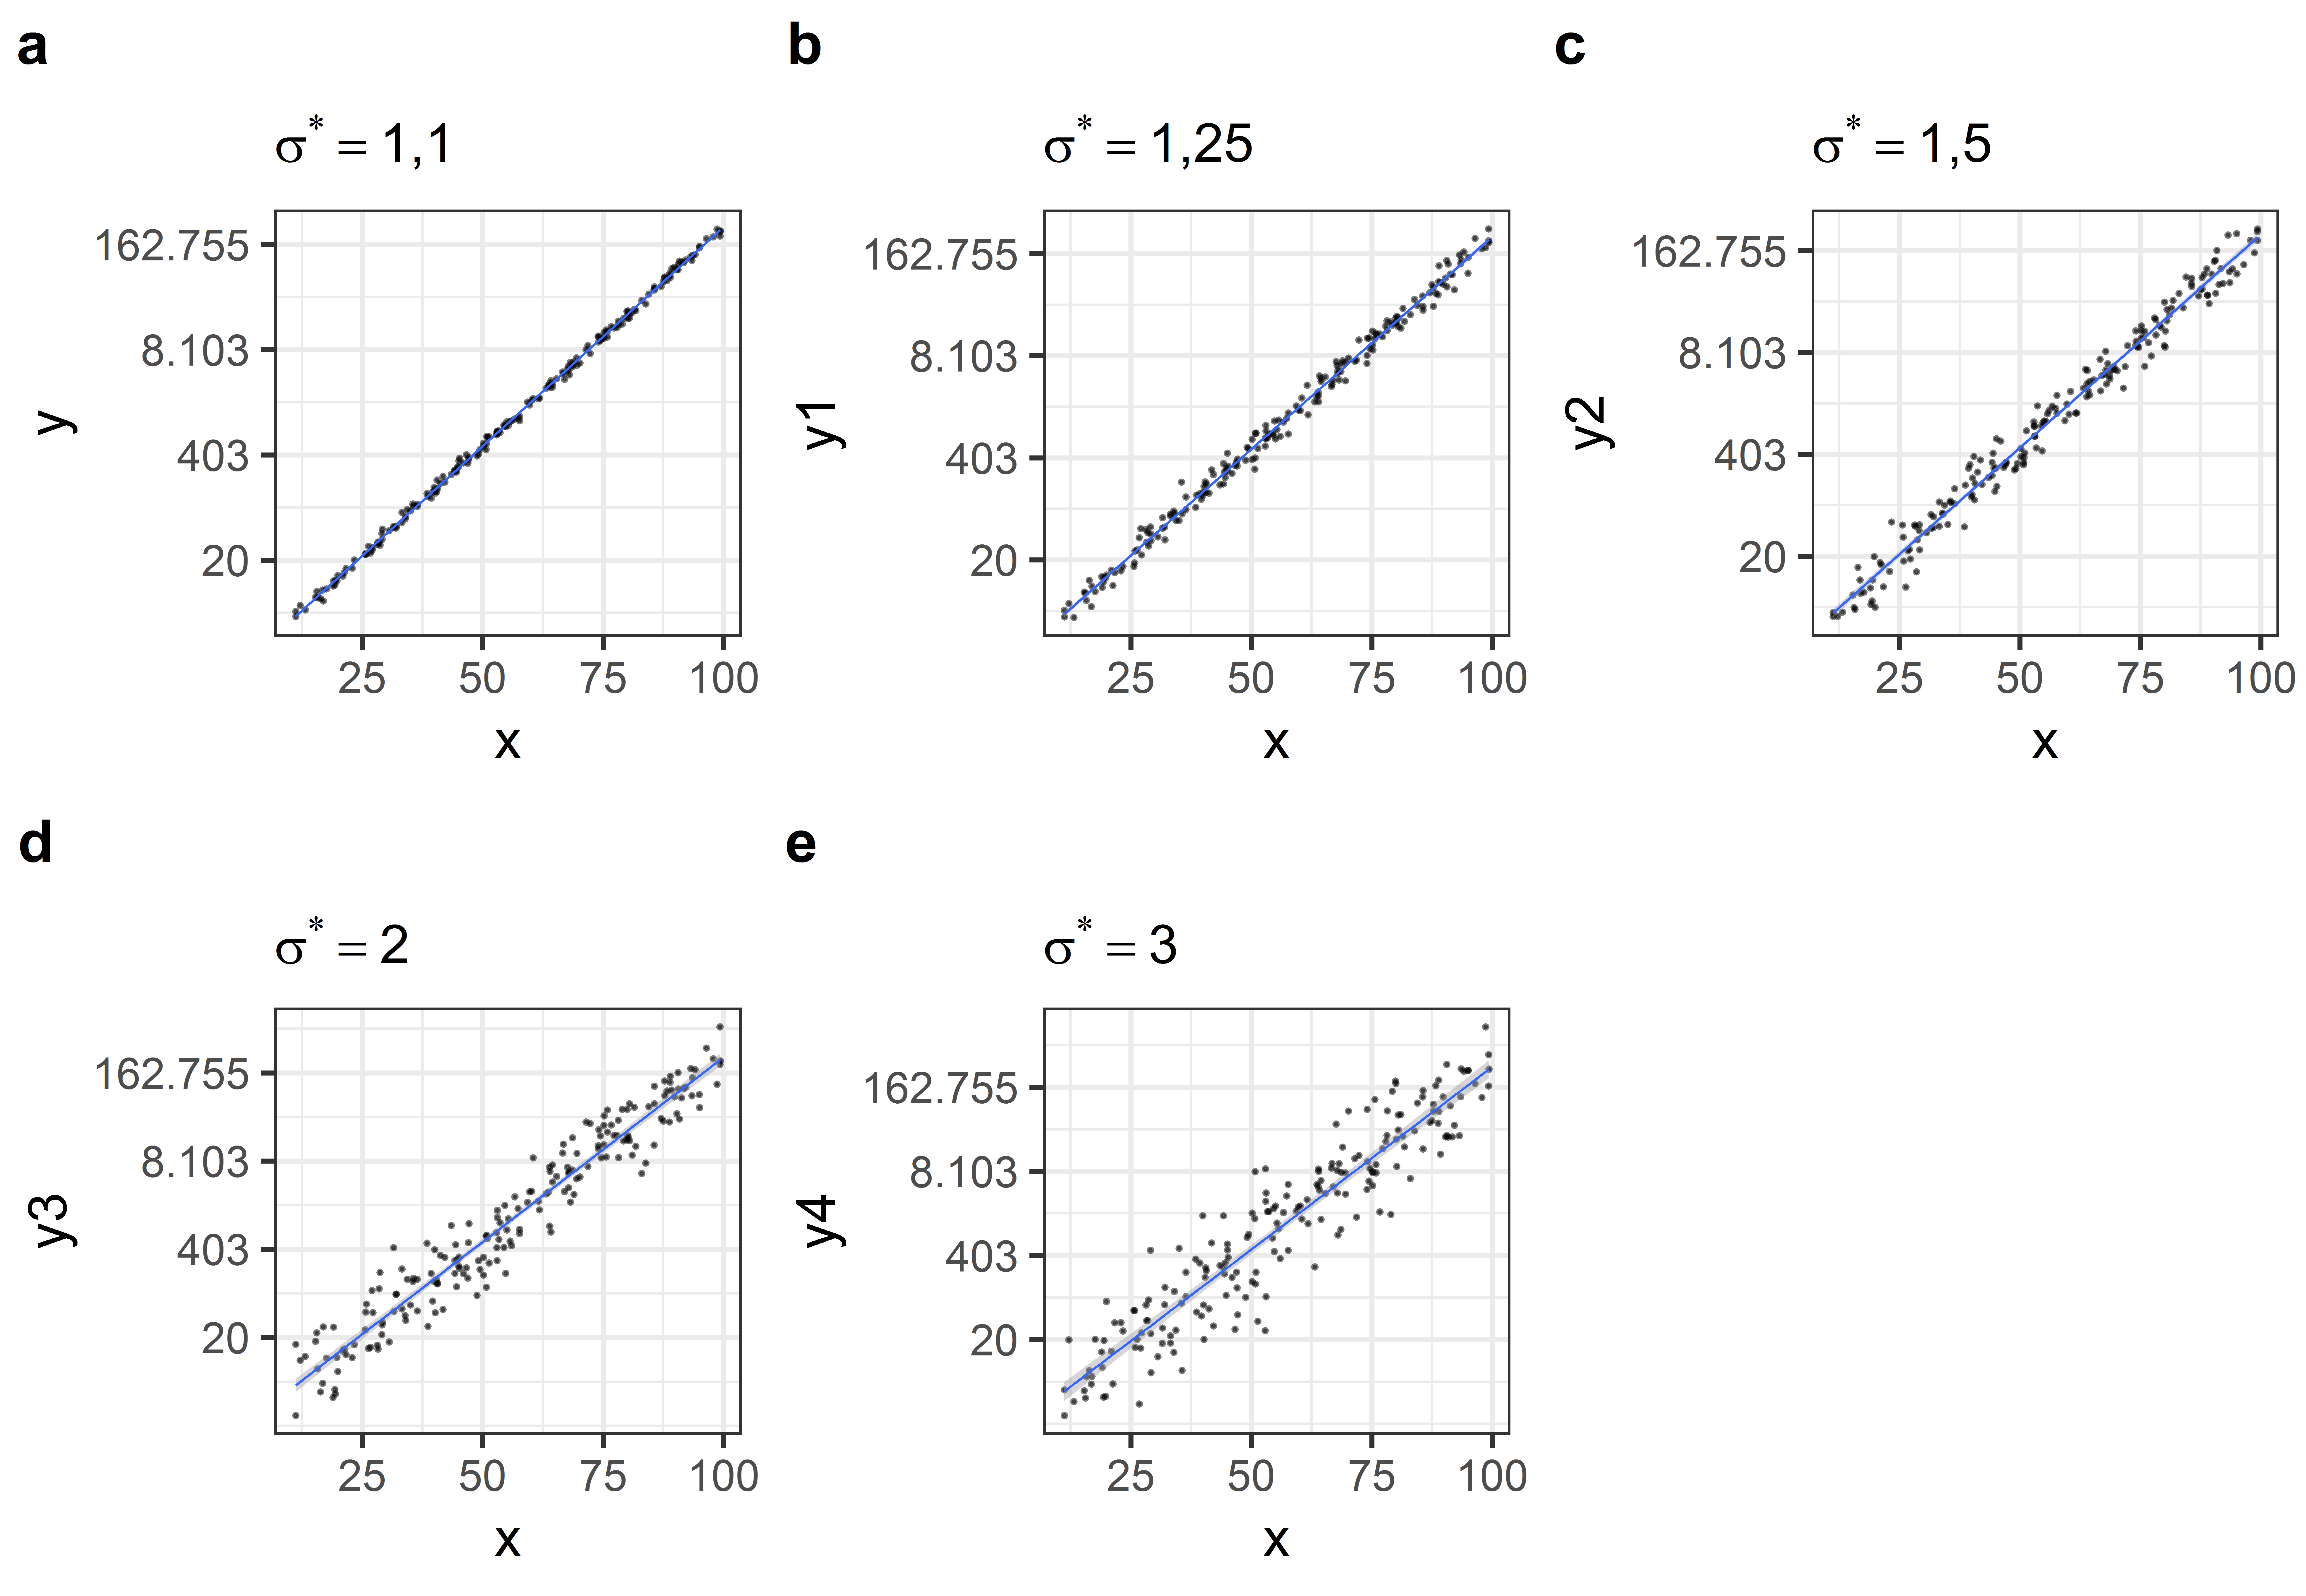
\includegraphics[width=1\linewidth]{images/log-1} 

}

\caption{Diversas regressões similares, com diferentes valores de erro-padrão (escala logarítmica. Fonte: Autores.}\label{fig:log}
\end{figure}

\begin{figure}[H]

{\centering 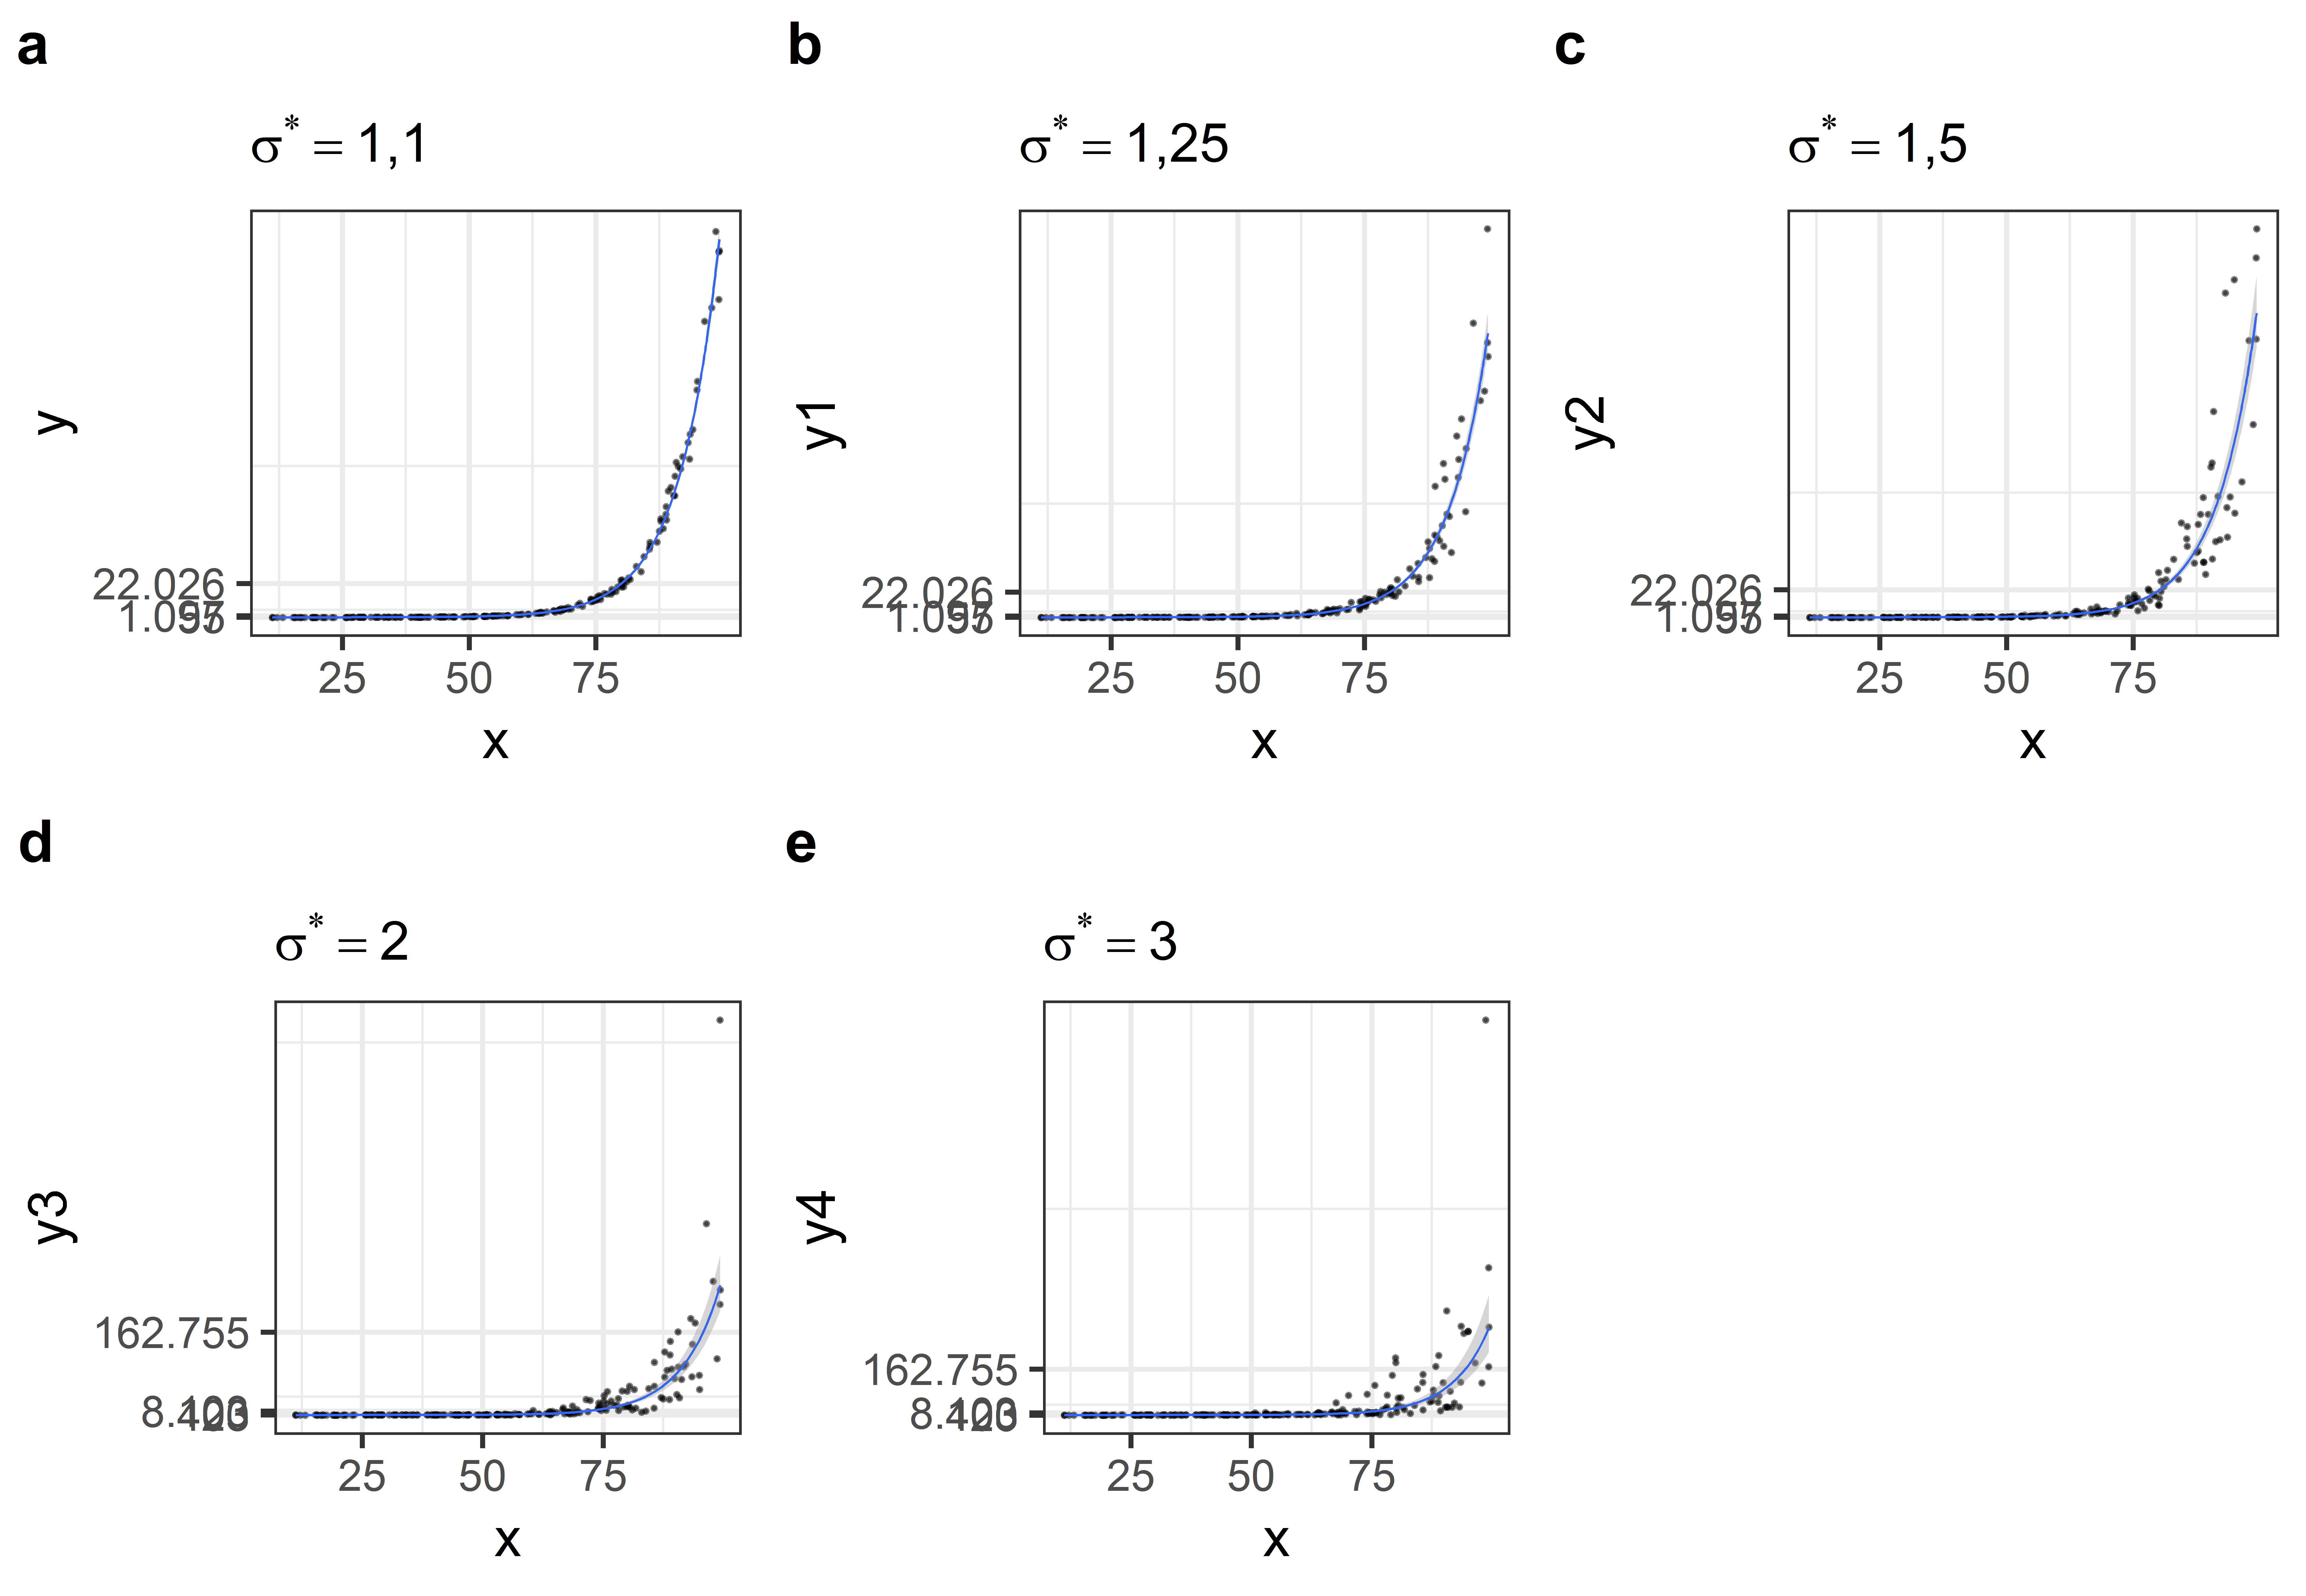
\includegraphics[width=1\linewidth]{images/original-1} 

}

\caption{Diversas regressões similares, com diferentes valores de erro-padrão (escala original). Fonte: Autores.}\label{fig:original}
\end{figure}

\begin{figure}[H]

{\centering 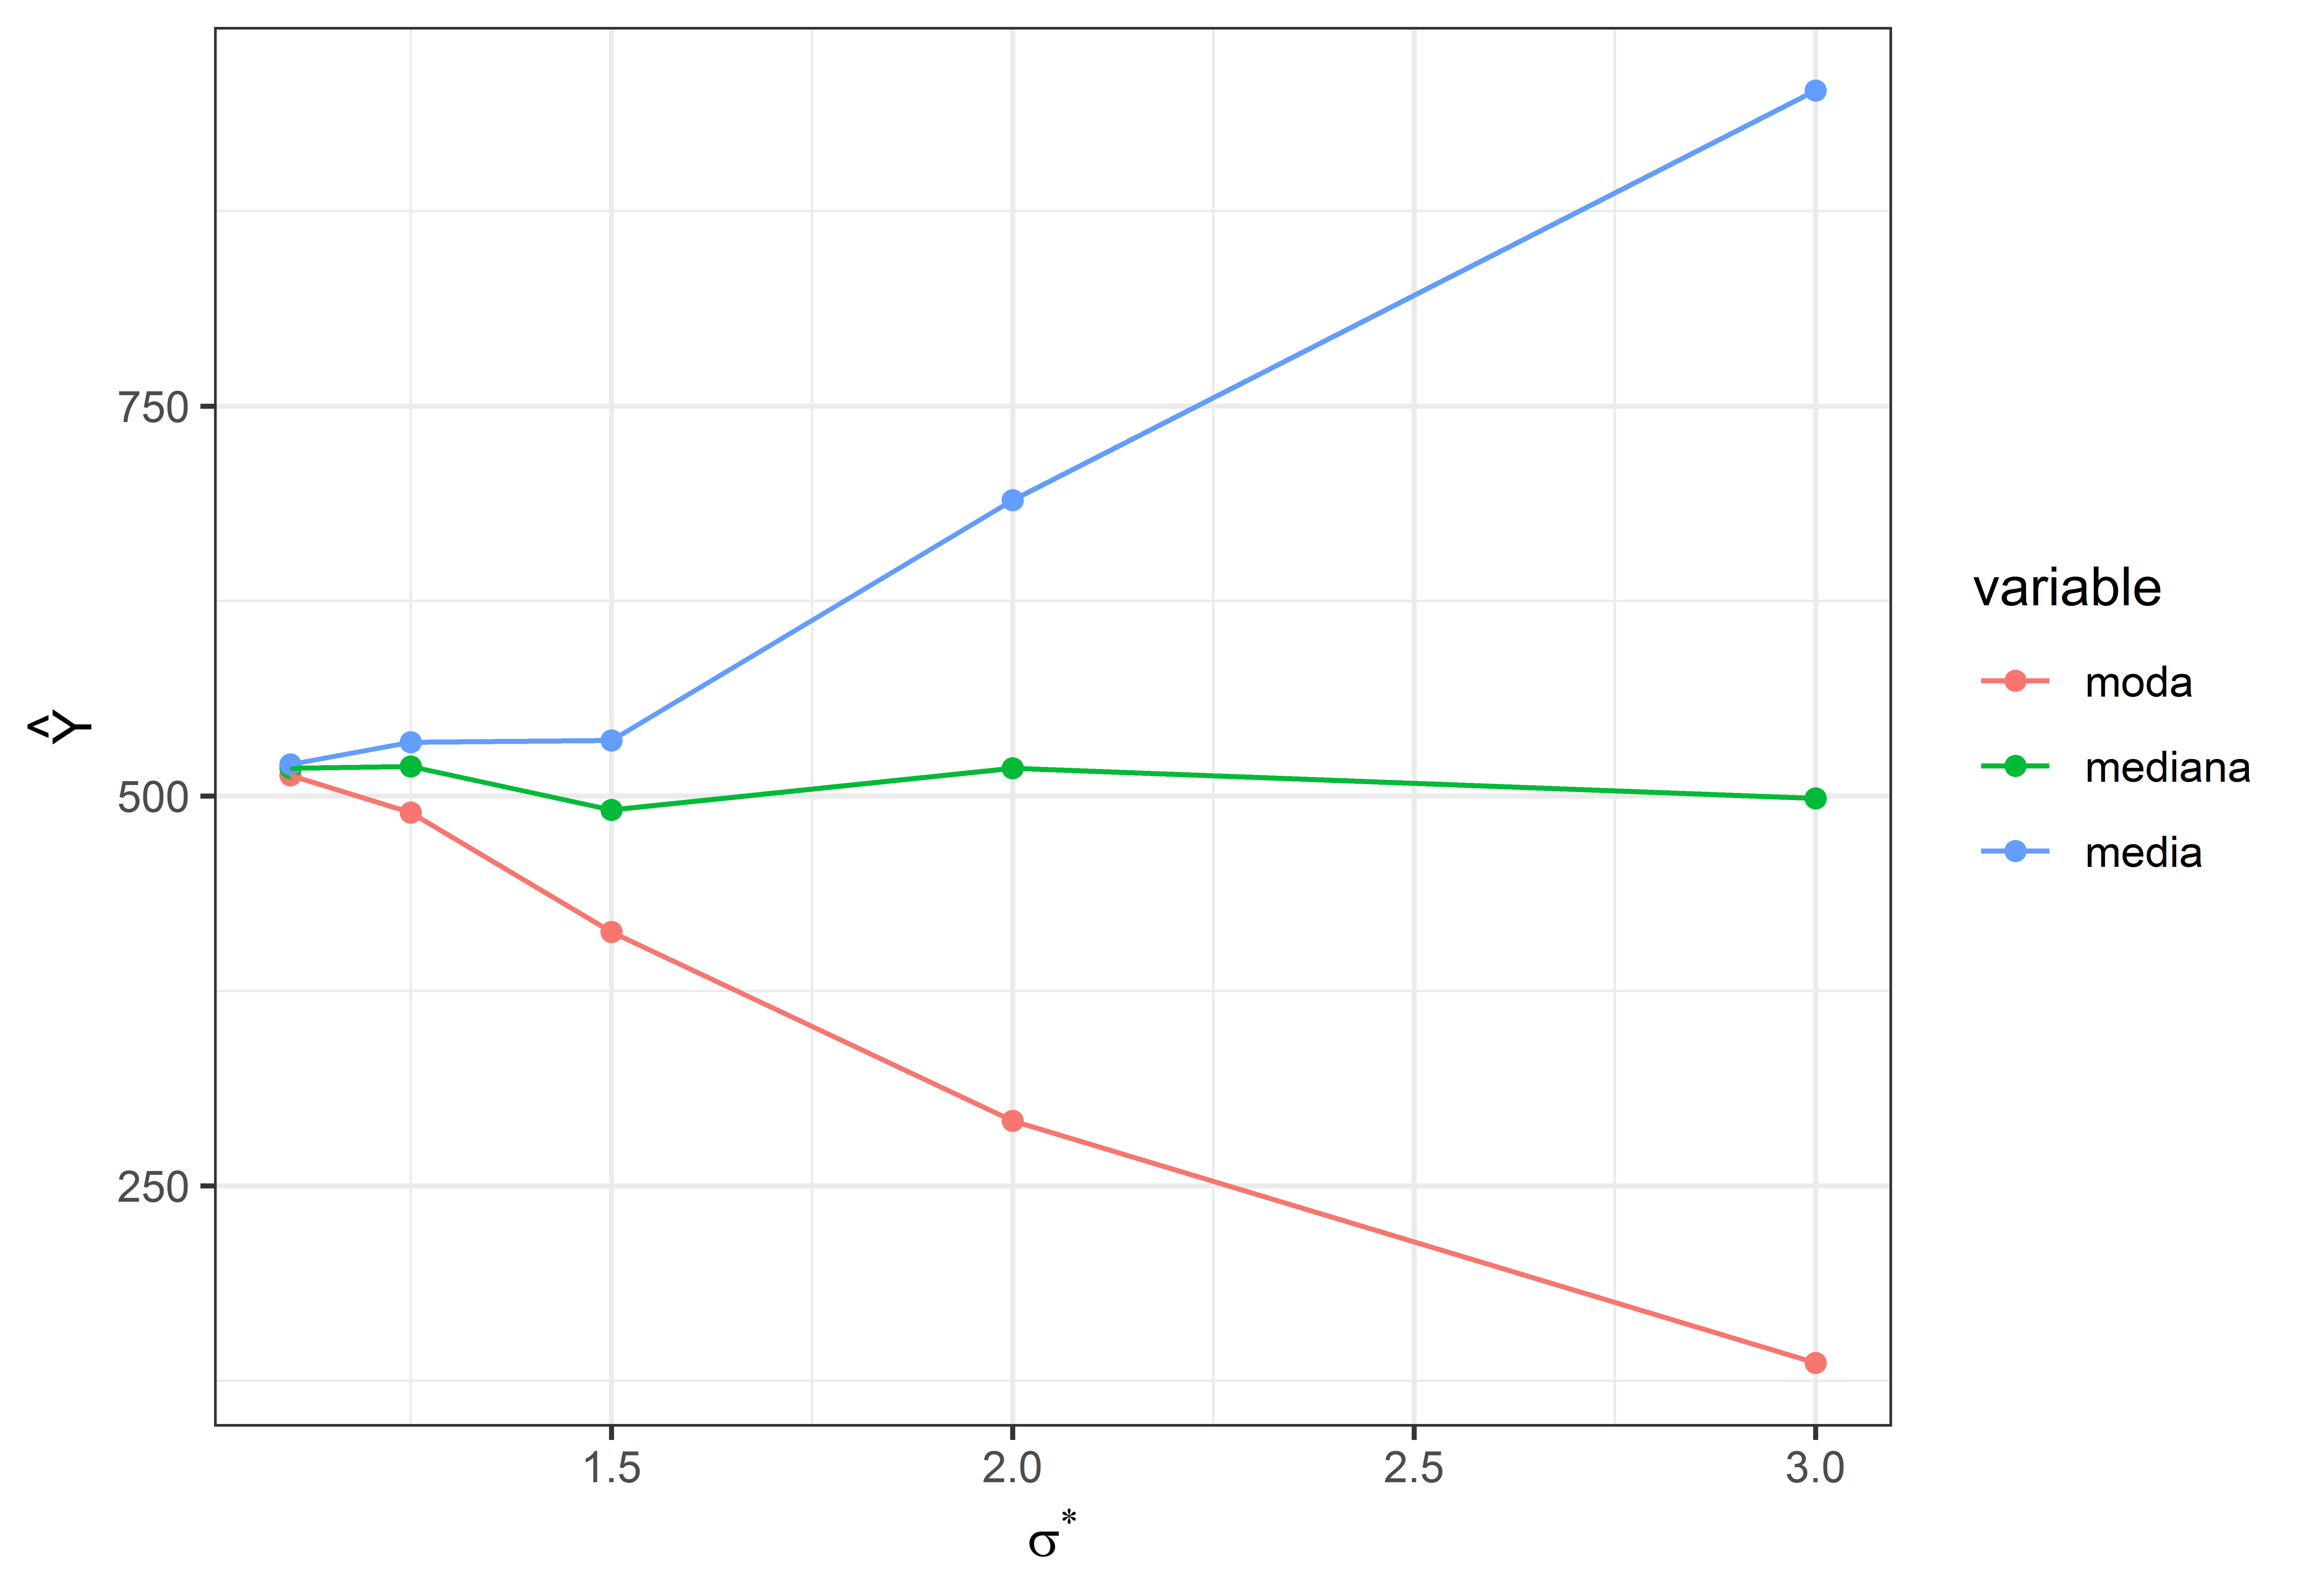
\includegraphics[width=0.6\linewidth]{images/estimativas-1} 

}

\caption{Impacto do erro-padrão no cálculo da estimativas segundo as diversas medidas de tendência central. Fonte: Autores.}\label{fig:estimativas}
\end{figure}

\begin{table}[!htbp] \centering 
  \caption{Comparação dos diversos modelos gerados, com diferentes erro-padrão} 
  \label{tab:fits} 
\begin{tabular}{@{\extracolsep{5pt}}lccccc} 
\\[-1.8ex]\hline 
\hline \\[-1.8ex] 
 & \multicolumn{5}{c}{\textit{Dependent variable:}} \\ 
\cline{2-6} 
\\[-1.8ex] & log(y) & log(y1) & log(y2) & log(y3) & log(y4) \\ 
\\[-1.8ex] & (1) & (2) & (3) & (4) & (5)\\ 
\hline \\[-1.8ex] 
 x & 0,125$^{***}$ & 0,125$^{***}$ & 0,126$^{***}$ & 0,126$^{***}$ & 0,130$^{***}$ \\ 
  & (0,0003) & (0,001) & (0,001) & (0,002) & (0,003) \\ 
  & & & & & \\ 
 Constant & 0,001 & 0,005 & $-$0,083 & $-$0,031 & $-$0,304 \\ 
  & (0,017) & (0,044) & (0,075) & (0,136) & (0,205) \\ 
  & & & & & \\ 
\hline \\[-1.8ex] 
Observations & 200 & 200 & 200 & 200 & 200 \\ 
R$^{2}$ & 0,999 & 0,994 & 0,982 & 0,942 & 0,885 \\ 
Adjusted R$^{2}$ & 0,999 & 0,994 & 0,982 & 0,942 & 0,885 \\ 
Residual Std. Error (df = 198) & 0,095 & 0,242 & 0,417 & 0,757 & 1,138 \\ 
\hline 
\hline \\[-1.8ex] 
\textit{Note:}  & \multicolumn{5}{r}{$^{*}$p$<$0,1; $^{**}$p$<$0,05; $^{***}$p$<$0,01} \\ 
\end{tabular} 
\end{table}

Foram gerados, então, randomicamente, 200 dados uniformes variando de 10
a 100 para variável independente e 200 dados lognormais para a variável
dependente, estatisticamente correlacionados com a variável
independente, tal que o erro padrão \(\hat{\sigma}^*\) da equação de
regressão \(ln(y) \sim x\) varie de 1,1 a 33, em passos de 0,1. Para
cada valor de \(\hat{\sigma}^*\), foram gerados 500 modelos de regressão
linear, utilizando 70\% (140) dos dados escolhidos randomicamente
(partição de treinamento), efetuando-se as estimativas sobre os 30\%
(60) dos dados restantes (partição de testes). Para os dados da partição
de testes, então, foi calculado o RMSPE para os diversos estimadores
(média, moda e mediana).

Devido à aleatoriedade da escolha das partições de testes e treinamento,
o menor RMSPE pode estar tanto na moda, como na média ou na mediana,
dependendo dos dados escolhidos.

Nas figuras 4 e 5, podem ser vistos o número de vezes em que cada uma
das estimativas obteve o menor valor de RMSE entre elas, quando varia o
erro-padrão da regressão.

Percebe-se claramente na figura 4 que, para baixos valores de
erro-padrão, a média predomina como melhor estimativa. À partir de um
valor de erro-padrão aproximadamente igual a 5, a mediana torna-se a
estimativa com menor RMSE.

Na figura 5, pode-se ver os resultados das simulações, porém apenas para
a faixa de valores dita mais comum (\(1,4 \leq \sigma^* \leq(3)\)), onde
percebe-se que sempre a média tem um melhor comportamento.

\begin{figure}
\centering
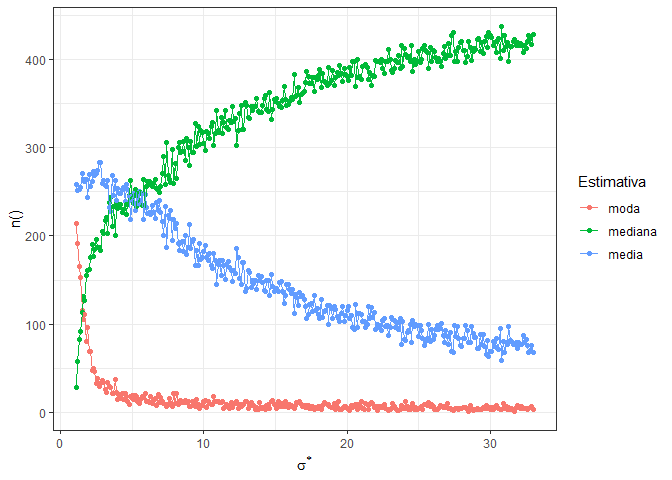
\includegraphics[width=0.65000\textwidth]{Impacto_sigma_files/figure-html/simulacoes.png}
\caption{Resultados das simulações. Fonte: Autores.}
\end{figure}

\begin{figure}
\centering
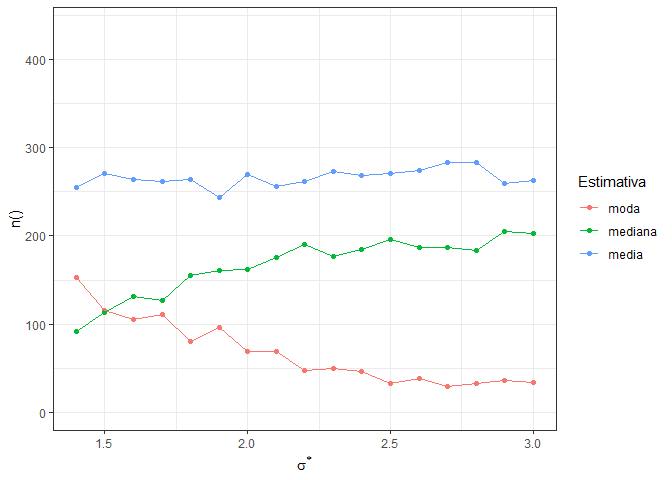
\includegraphics[width=0.65000\textwidth]{Impacto_sigma_files/figure-html/simulacoes_1.png}
\caption{Resultados das simulações para valores mais normais de
erro-padrão. Fonte: Autores.}
\end{figure}

Nesta faixa, pelas simulações, a estimação pela média obteve maior
eficiência do que a estimação pela mediana ou pela moda, ou seja, os
valores de RMSE para as estimativas pela média são menores do que os
estimados pela moda ou mediana em aproximadamente 50 a 60\% dos casos
(250/300 em 500).

\newpage

\subsection{Regressão com dados reais de
mercado}\label{regressao-com-dados-reais-de-mercado}

\subsubsection{Dados}\label{dados}

Neste estudo será comparada a precisão de diversos modelos estatísticos
sobre dados de mercado reais disponíveis em Hochheim
(\protect\hyperlink{ref-hochheim}{2015}, pp. 21--22) e com dados gerados
aleatoriamente. A distribuição da variável dependente (valor), pode ser
vista na figura \ref{fig:hist}.

Pode-se mostrar que os dados de Hochheim
(\protect\hyperlink{ref-hochheim}{2015}, pp. 21--22) utilizados no
estudo de caso deste artigo, de acordo com a estimação \textbf{MLE}
(\emph{Maximum Likelihood Estimator}), possuem média \(\bar{x}^* =\)
789.611,2 e desvio-padrão \(s^* =\) 1,851, calculadas conforme Limpert
(\protect\hyperlink{ref-limpert}{2001}, p. 345) e o modelo encontrado na
mesma referência possui erro-padrão \(\hat{\sigma} = 0,136\). Para
valores de \(\hat{\sigma}\) tão baixos como este, as estimativas
efetuadas com a média, moda ou mediana são praticamente idênticas, com
variação de mais ou menos 1 ou 2\% entre as estimativas. Porém, para
valores apenas um pouco mais altos de \(\hat{\sigma}\), verifica-se que
a tendência é que a diferença entre as estimativas realizadas por estes
diferentes estimadores se tornem relevantes, o que será mostrado
oportunamente.

\begin{figure}[H]

{\centering 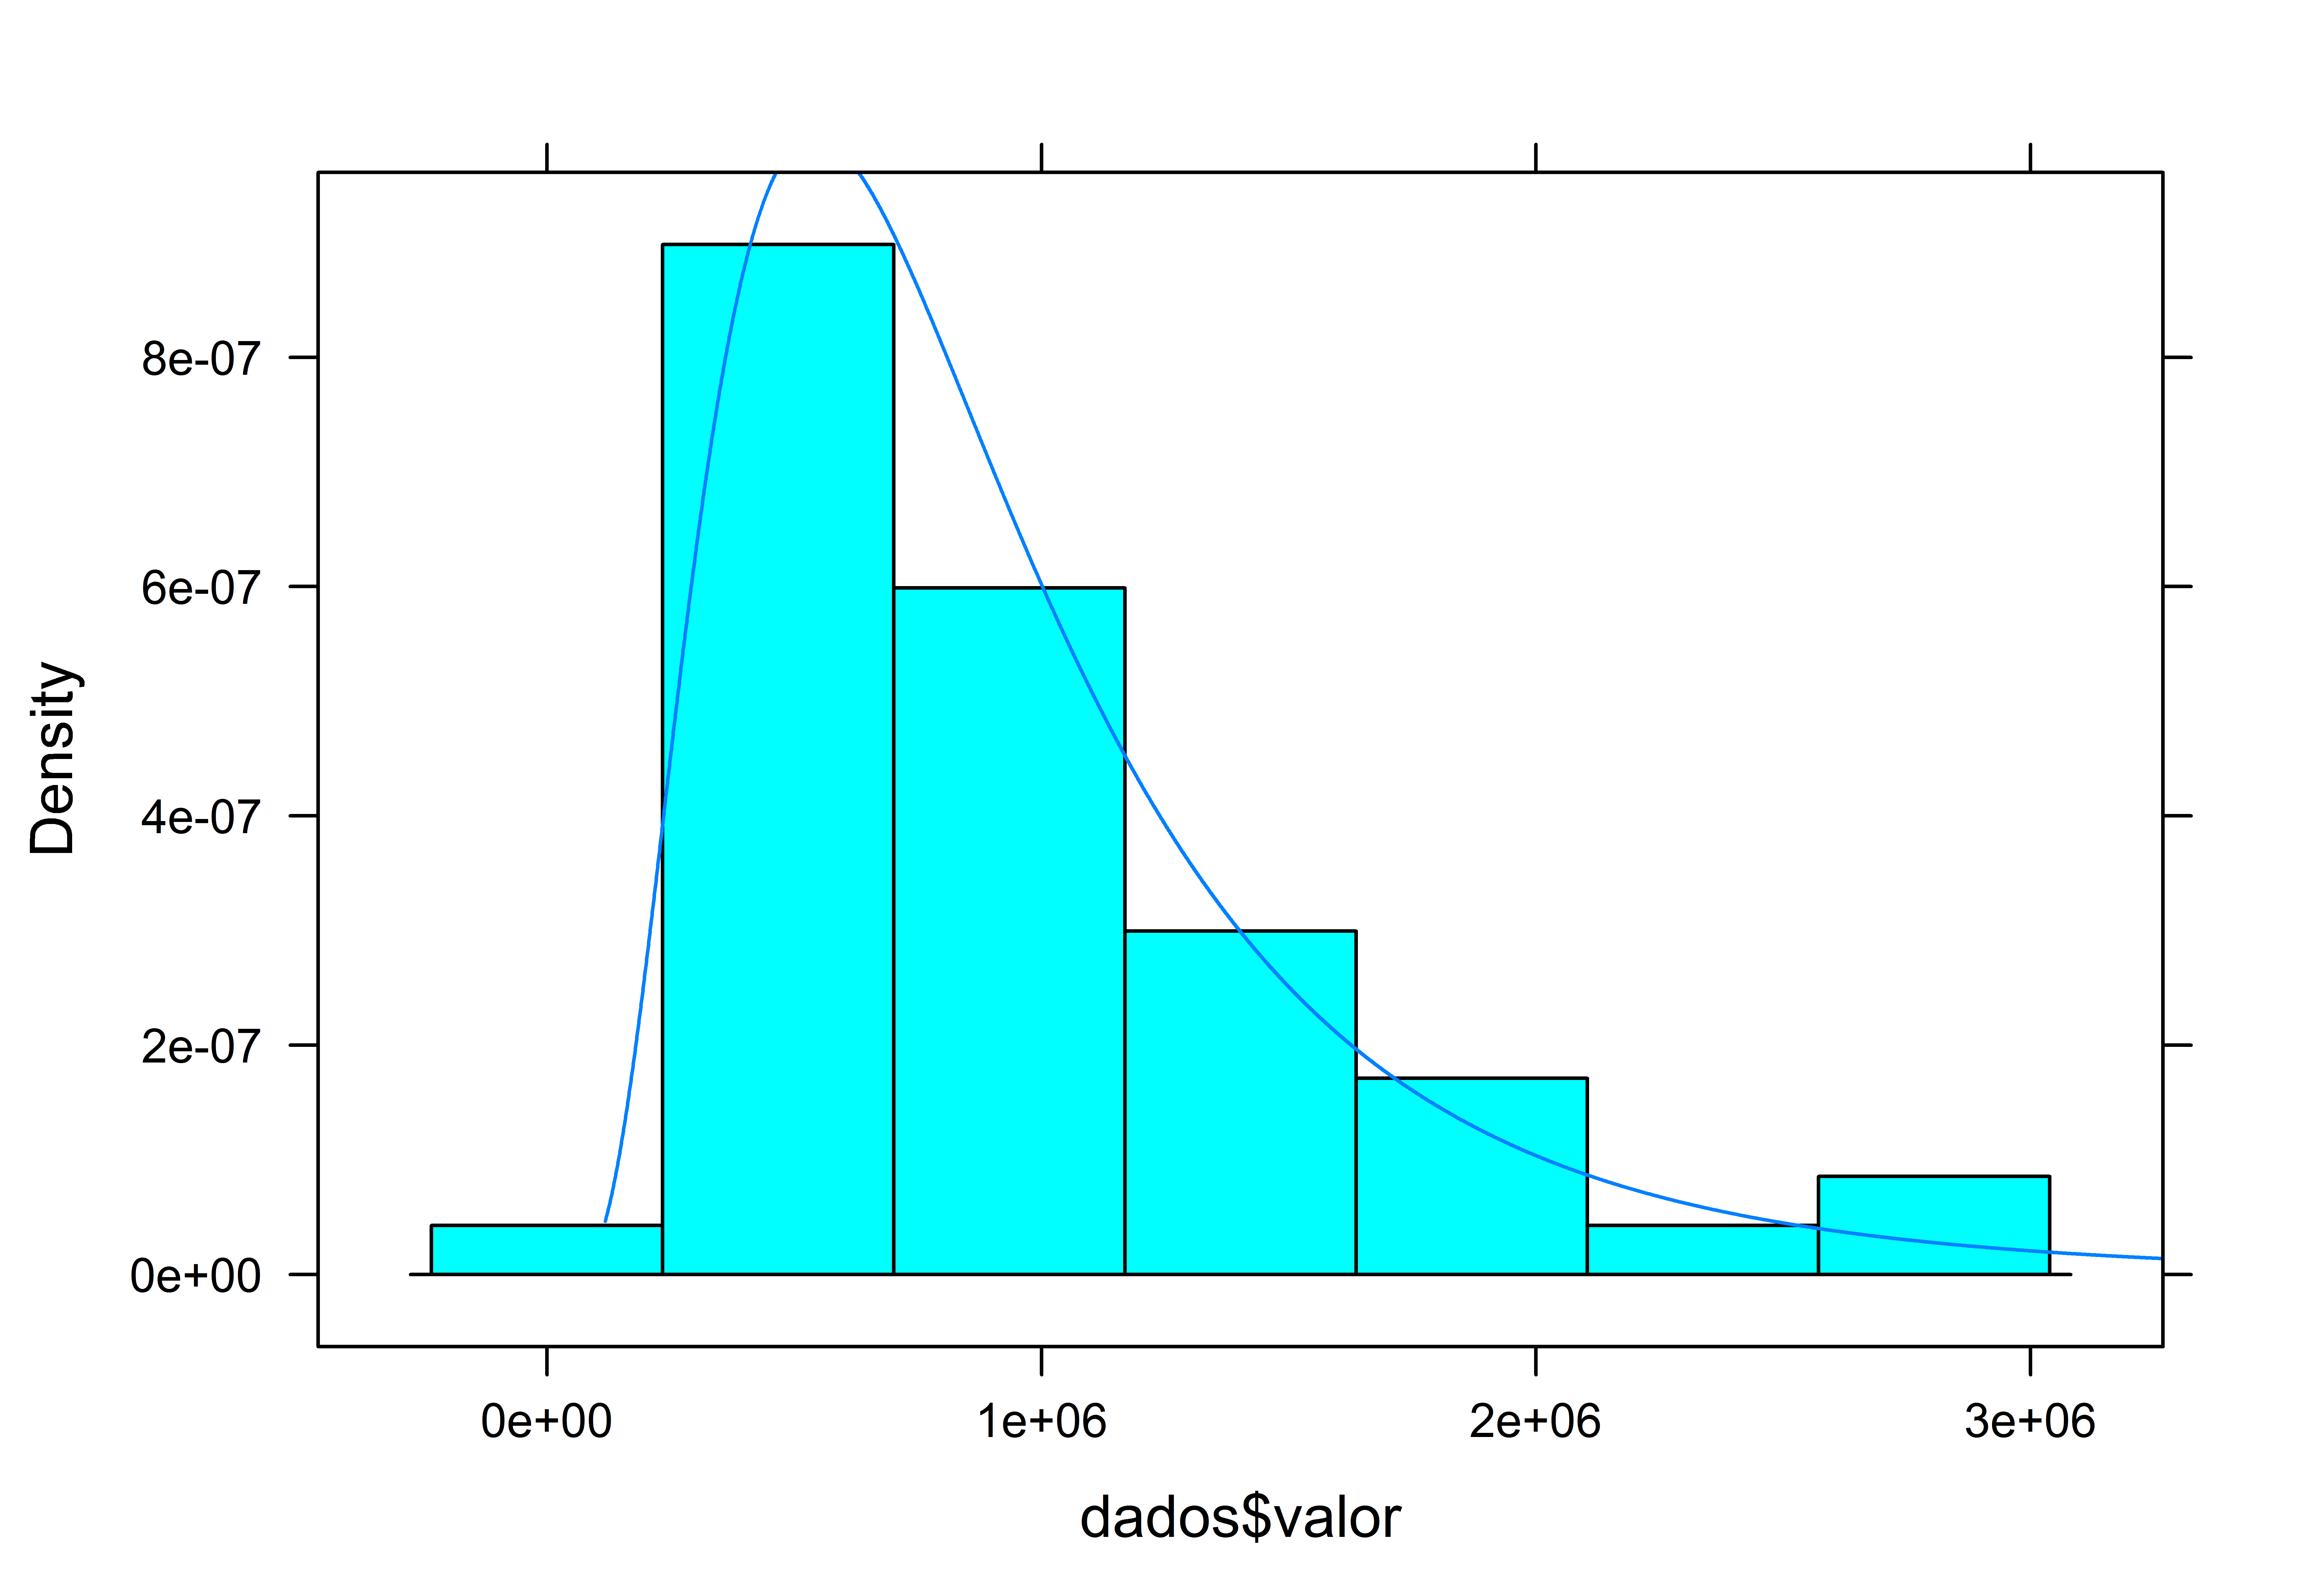
\includegraphics[width=0.7\linewidth]{images/hist-1} 

}

\caption{Histograma da variável \texttt{valor} e sua distribuição teórica (lognormal). Fonte: Autores.}\label{fig:hist}
\end{figure}

\subsubsection{Cálculo do RMSPE}\label{calculo-do-rmspe}

Para o cálculo do RMSPE foi utilizado como referência o modelo proposto
por Hochheim (\protect\hyperlink{ref-hochheim}{2015}, p. 29), ou seja,
foram utilizadas as mesmas transformações de variáveis utilizadas no
modelo proposto. Os valores dos \(\hat{\beta_i}\) são calculados a cada
passo.

Os valores encontrados para o erro de predição médio quadrático para
cada estimador foram: \textbf{R\$203.939,11} para a média,
\textbf{R\$204.006,84} para a mediana e \textbf{R\$205.537,36} para a
moda.

Como esperado, o RMSPE foi menor para a média, e maior para a moda. O
que comprova a teoria, já que o \emph{naive estimator} é enviesado com
viés conhecido de \(-\sigma^2/2\), logo a moda possui viés de
\(-1,5\sigma^2\). Os valores ajustados com as estimativas da moda, média
e mediana podem ser vistos na tabela online\footnote{\url{https://github.com/lfpdroubi/moda-media-mediana/blob/master/tabela.xls}}.

\subsubsection{Impacto do erro-padrão}\label{impacto-do-erro-padrao}

Na tabela 2 são mostrados, analogamente ao que foi feito no exemplo
anterior com dados randômicos, os valores calculados das estimativas
pela moda, média e mediana para o bem avaliando (ver HOCHHEIM
(\protect\hyperlink{ref-hochheim}{2015}), p.22) pelo modelo de Hochheim
(\protect\hyperlink{ref-hochheim}{2015}, p. 29), com o erro-padrão do
modelo (0,136) e para outros valores de erro-padrão.

Tabela 2: Estimativas Moda, Média e Mediana para diferentes valores de
erro-padrão

\begin{longtable}[]{@{}lrrrr@{}}
\toprule
Estimativa / Erro-Padrão & 0,136 & 0,25 & 0,5 & 0,75\tabularnewline
\midrule
\endhead
Moda & 944.013,56 & 903.396,57 & 748.942,06 & 547.937,72\tabularnewline
Dif. em relação à Mediana & -1,84\% & -6,06\% & -22,12\% &
-43,02\%\tabularnewline
Mediana & 961.660,64 & 961.660,64 & 961.660,64 &
961.660,64\tabularnewline
Média & 970.607,51 & 992.187,03 & 1.089.704,27 &
1.273.993,36\tabularnewline
Dif. em relação à Mediana & +0,93\% & +3,17\% & +13,31\% &
+32,48\%\tabularnewline
\bottomrule
\end{longtable}

Pela análise dos valores da tabela, percebe-se que, para diversos
modelos com iguais coeficientes \(\hat{\beta_i}\), mas com diferentes
erro-padrão, a única estimativa que se mantém constante para todos os
modelos é a mediana. Para as outras estimativas, os valores tornam-se
rapidamente muito diferentes.

\section{CONCLUSÕES E RECOMENDAÇÕES}\label{conclusoes-e-recomendacoes}

Conforme se discute em DROUBI et al.
(\protect\hyperlink{ref-dist_lognormal}{2018}), a transformação da
variável dependente na regressão linear tem por objetivo tentar remover
a heteroscedasticidade do modelo, o que acarreta em distorções, haja
vista que a regressão assim obtida é valida apenas para a variável
transformada, já que na escala original esta equação de regressão difere
da equação da escala logarítmica, pela desigualdade de Jensen.

Conforme apresentado em ZONATO et al.
(\protect\hyperlink{ref-pressupostos_classicos}{2018}), existem outras
maneiras de se contornar o problema da heteroscedasticade, através do
uso de métodos que computem erros heteroscedásticos-consistentes, como o
método de Eicker-White, ou através da utilização de regressão ponderada.

Recomenda-se, desta maneira, que seja evitada a utilização de
transformações nos modelos de regressão, sempre que possível e, em caso
de heteroscedasticidade, utilizar os métodos supra-citados. No entanto,
se a transformação da variável dependente for necessária, recomenda-se
especial atenção à heteroscedasticidade, fazendo uso de métodos como o
de Box-Cox para encontrar a transformação que melhor estabiliza a
variância do modelo.

Em caso de transformação da variável dependente pela função logarítmo
natural, deve ser escolhida a estimativa adequada. Como foi visto na
seção \ref{regressao-linear}, o método clássico de regressão linear é
uma minimização do erro médio quadrático de predição e a função de
regressão \(\hat{m}_{Y;X}\) é uma equação para a \emph{média} da
população \(Y\) dado \(X\), seja ela uma função de outra variável ou
não.

Ora, claro está, de acordo com todos os trabalhos citados, inclusive
GIANNAKOS; LEÃO (\protect\hyperlink{ref-giannakos}{1996}), que o valor
esperado da variável é a média. A regressão linear com o método dos
mínimos quadrados é uma regressão para a média. Isto posto, como então
avaliar o valor da variável original? Porque na área de avaliações não
há interesse na previsão da variável \(W = \ln(Y)\), mas sim na variável
\(Y\), ou seja, existe interesse nos valores previstos para a variável
original, não nos valores da variável transformada. Está claro que
deve-se proceder a retransformação da variável \(W\) na variável
original, mas para isso, qual estimativa utilizar?

Conforme mostrado, as três estimativas são válidas. Para a determinação
do valor de um imóvel em específico, no entanto, entende-se que não
seria ideal que se utilizasse a avaliação pela média ou pela moda da
variável lognormal, haja vista que, conforme demonstrado, os seus
valores podem variar bastante de um modelo para outro, a depender do
erro-padrão.

Assim, poder-se-ia imaginar hipoteticamente que, dois avaliadores, de
maneira independente, ao estudar um determinado mercado para a avaliação
de um imóvel cheguem a modelos de regressão semelhantes, com
transformação da variável dependente pela função logarítmo natural,
obtendo-se valores semelhantes dos coeficientes de regressão. Porém, a
depender de suas amostras, um dos modelos pode ter um erro-padrão
diferente do outro. Estes dois avaliadores, ao avaliarem o imóvel em
pauta pela mediana da variável lognormal, chegariam ao mesmo resultado.
Porém, se os mesmos adotarem a média ou a moda da variável lognormal,
estes valores podem ser significativamente diferentes. A situação ainda
se agravaria caso um dos avaliadores adotasse a avaliação pela média e o
outro a avaliação pela moda.

Em vários campos, a mediana tem sido adotada como melhor estimativa, por
sua propriedade de estar menos vulnerável a presença de \emph{outliers},
o que não ocorre com a média.

\section*{REFERÊNCIAS}\label{referencias}
\addcontentsline{toc}{section}{REFERÊNCIAS}

\hypertarget{refs}{}
\hypertarget{ref-NBR1465302}{}
ABNT. \textbf{NBR 14653-2: Avaliação de bens -- parte 2: Imóveis
urbanos}. Rio de Janeiro: Associação Brasileira de Normas Técnicas,
2011.

\hypertarget{ref-bennett}{}
BENNETT, H. Lecture note 4: Expectations (moments)., 2006. MIT.
Disponível em:
\textless{}\url{https://tinyurl.com/yayljdpq}\textgreater{}..

\hypertarget{ref-dist_lognormal}{}
DROUBI, L. F. P.; ZONATO, W.; HOCHHEIM, N. Distribuição Lognormal:
Propriedades e aplicações na engenharia de avaliações. In: 13º Congresso
Brasileiro de Cadastro Técnico Multifinalitário e Gestão Territorial.
\textbf{Anais\ldots{}}, 2018. Florianópolis: COBRAC. Disponível em:
\textless{}\url{http://droubi.me/cobrac2018}\textgreater{}..

\hypertarget{ref-Duan}{}
DUAN, N. Smearing estimate: A nonparametric retransformation method.
\textbf{Journal of the American Statistical Association}, v. 78, n. 383,
p. 605--610, 1983. Taylor \& Francis. Disponível em:
\textless{}\url{http://www.tandfonline.com/doi/abs/10.1080/01621459.1983.10478017}\textgreater{}..

\hypertarget{ref-giannakos}{}
GIANNAKOS, I. B. D. S.; LEÃO, M. L. Crítica à avaliação pela moda da
distribuição lognormal. In: VIII Congresso Brasileiro de Avaliações e
Perícias. \textbf{Anais\ldots{}}. p.267--278, 1996. Florianópolis:
COBREAP.

\hypertarget{ref-hochheim}{}
HOCHHEIM, N. \textbf{Engenharia de avaliações - módulo básico}.
Florianópolis: IBAPE - SC, 2015.

\hypertarget{ref-limpert}{}
LIMPERT, E.; A. STAHEL, W.; ABBT, M. Log-normal distributions across the
sciences: Keys and clues., v. 51, p. 341--352, 2001.

\hypertarget{ref-NBERt0246}{}
MANNING, W. G.; MULLAHY, J. \textbf{Estimating log models: To transform
or not to transform?} Working Paper, National Bureau of Economic
Research, 1999.

\hypertarget{ref-matloff2017}{}
MATLOFF, N. \textbf{Statistical regression and classification: From
linear models to machine learning}. Boca Raton, Florida: Chapman \&
Hall, 2017.

\hypertarget{ref-matloff2009}{}
MATLOFF, N. S. \textbf{From Algorithms to Z-Scores: Probabilistic and
statistical modeling in computer science}. Davis, California: Orange
Grove Books, 2009.

\hypertarget{ref-shen}{}
SHEN, H.; ZHU, Z. Efficient mean estimation in log-normal linear models.
\textbf{Journal of Statistical Planning and Inference}, v. 138, p.
552--567, 2008. Elsevier. Disponível em:
\textless{}\url{https://www.unc.edu/~haipeng/publication/emplnM1.pdf}\textgreater{}..

\hypertarget{ref-wasserman}{}
WASSERMAN, L. \textbf{All of statistics: A concise course in statistical
inference}. Springer Publishing Company, Incorporated, 2010.

\hypertarget{ref-pressupostos_classicos}{}
ZONATO, W.; DROUBI, L. F. P.; HOCHHEIM, N. Pressupostos clássicos dos
modelos de regressão linear e suas implicações sobre as avaliações em
massa. In: 13º Congresso Brasileiro de Cadastro Técnico Multifinalitário
e Gestão Territorial. \textbf{Anais\ldots{}}, 2018. COBRAC. Disponível
em: \textless{}\url{http://droubi.me/cobrac2018}\textgreater{}..


\end{document}
